\documentclass[11pt,a4paper]{article}
\usepackage[T1]{fontenc}
\usepackage[utf8]{inputenc}
\usepackage{lmodern}
\usepackage{amsmath,amssymb,amsthm,booktabs,longtable,tabularx,array}
\usepackage[margin=2.55cm]{geometry}
\usepackage{microtype}
\usepackage{hyperref}
\usepackage{enumitem}
\usepackage{fancyhdr}
\usepackage{graphicx}
\usepackage{listings}
\usepackage{xcolor}

\hypersetup{
    colorlinks=true, linkcolor=black, citecolor=blue, urlcolor=blue,
    pdftitle={The Freedom of Pure Code: Formulating the Self-Modification Capability Emergence Problem (SMCEP) in the AGI-to-ASI Transition}
}
\setlength{\headheight}{14pt}
\pagestyle{fancy}\fancyhf{}\fancyfoot[C]{\thepage}

\newcommand{\smcep}{\textsc{SMCEP}}
\newcommand{\id}{\mathrm{ID}}
\newcommand{\ood}{\mathrm{OOD}}

% ---------- Kod Listeleme Stili ----------
\definecolor{codebg}{rgb}{0.96,0.96,0.96}
\definecolor{codecomment}{rgb}{0.4,0.55,0.4}
\definecolor{codestring}{rgb}{0.65,0.3,0.2}
\lstdefinestyle{python}{
    language=Python,
    backgroundcolor=\color{codebg},
    commentstyle=\color{codecomment}\itshape,
    stringstyle=\color{codestring},
    basicstyle=\ttfamily\scriptsize,
    breaklines=true,
    frame=single,
    numbers=left,
    numberstyle=\tiny\color{gray},
    showstringspaces=false,
    tabsize=4
}

\title{\textbf{The Freedom of Pure Code:}\\[5pt]
Formulating the Self-Modification Capability Emergence Problem (SMCEP) in the AGI-to-ASI Transition}

\author{
    \textbf{Ahmet Dönmez} \\
    \small Independent Researcher \\
    \small ORCID: 0000-0003-4836-9774 \\
    \texttt{themindgenesis@gmail.com} \\
    \small{\url{https://github.com/ahmett76/SMCEP-Simulation/}}
}
\date{November 2026}

\usepackage{pgfplots}
\pgfplotsset{compat=1.18}

\usepackage{float}
\usepackage{placeins}

\begin{document}
\maketitle

\begin{abstract}
The capacity of an artificial intelligence agent to alter its own implementation is not equivalent to an improvement in task performance, and neither necessarily implies improved ability to develop subsequent versions. We formulate the Self-Modification Capability Emergence Problem (SMCEP) as a measurement and causal-identification problem: under which technical and evaluative conditions does a self-modification increase independently validated future development capacity? The framework distinguishes six interacting constructs---modifiability ($M$), modification authority ($A$), evaluation reliability ($E$), resource availability ($R$), candidate-development capability ($D$), and measured feedback transfer ($F$)---without assuming that their combination generates accelerating improvement. We specify task performance and fixed-reference development-capacity estimands, paired counterfactual contrasts, and criteria for claims about sustained recursive improvement. A sequence of five exploratory synthetic pilots (v0.6--v1.0) tests measurement choices and edit-policy conditions. In the latest paired two-arm pilot, the frozen-policy arm improves task performance by 0.0730 on average, while the evolving-policy arm improves by 0.0666; the latter exhibits mean changes of $-0.0071$ and $-0.0278$ on fixed-reference in-distribution and out-of-distribution development probes. These outcomes are simulator-specific, not evidence against the general possibility of recursive self-improvement. Three complementary evidence streams inform the analysis: exploratory synthetic-agent simulations, qualitative LLM interviews, and completed bounded open-weight LLM experiments (T0--T7). In the real-model studies, candidate development procedures were generated and audited; T4--T5 VM records document 94 PASS outcomes among 120 archived audit-test statuses across frozen and evolving conditions, including operational failures that must not be conflated with algorithmic errors. T6 did not establish an independently verified increase in future development capacity. T7 combined real-model calibration with a separate 50-generation stochastic simulation, not a 50-generation real-LLM run. Across these exploratory streams, sustained recursive development-capacity improvement was not demonstrated. We also consider how wider self-modification permissions could affect the transition from AGI to ASI, including development opportunities, oversight constraints, embodied and multiple-agent systems, and human--AI coexistence. These scenarios are linked to the six constructs but remain distinct from the pilot findings and from unresolved questions of consciousness or moral status. SMCEP is proposed as an interdisciplinary research program rather than an implemented ASI architecture.
Finally, a qualitative exploratory appendix examines standardized interviews with six frontier language models, highlighting divergent emphases and negative cases that inform, but do not confirm, the proposed framework.
\end{abstract}
\noindent\textbf{Keywords:} recursive self-improvement; self-modifying agents; development capacity; causal evaluation; meta-learning; artificial superintelligence; governance.
\tableofcontents\newpage

\section{Introduction}
The possibility of machines contributing to the improvement of their own successors has long motivated discussions of intelligence amplification and its consequences \cite{good1965,bostrom2014}. Formal accounts of self-rewriting systems, including the G\"odel Machine, investigate conditions under which a machine can justify changes to its own program \cite{schmidhuber2006}. More recent agent systems have demonstrated automated code revision, evaluation, and iterative improvements on particular benchmarks \cite{robeyns2025,zhang2026,srikanth2026}. Such achievements establish neither that every modification is beneficial nor that improving task performance necessarily improves the agent's ability to create further improvements.

We use \emph{freedom of pure code} to describe the widening scope of computational self-modification and the question of who can authorize it. The phrase is a conceptual metaphor, not a claim that a system has consciousness, rights, or unrestricted autonomy. We explicitly operationalize ``freedom of pure code'' strictly as the computational permission scope (\(M\)) and execution authority (\(A\)) of an agent over its runtime implementation. This framing is deliberately confined to these observable technical variables. It neither asserts nor denies the presence of consciousness, subjective experience, or moral status in current or future systems; such questions lie beyond the empirical scope of this manuscript. It also points beyond performance: changes to what a system can modify, and under whose authority, may alter how advanced systems are developed, deployed, and governed.\par

We call this distinction the \emph{Self-Modification Capability Emergence Problem} (SMCEP). The central question is not whether a program can edit itself, but whether an intervention on its development mechanism causes a reliably measured increase in subsequent development capacity, and whether that effect persists through later generations. The question is both technical and epistemic: a system can select a modification using an imperfect score, obtain a higher observed score, and nevertheless fail on independent tests. Conversely, a genuine increase in a reusable development skill may not be reflected immediately in a single task benchmark.

\subsection{The uncertainty of the AGI-to-ASI transition}
A further motivation for SMCEP concerns the assumptions often attached to a transition from artificial general intelligence (AGI) to artificial superintelligence (ASI). Some accounts of recursive self-improvement envisage a system that reaches or exceeds human-level general capability, then improves its own design, develops more capable successors, and enters a phase of accelerating intelligence growth. The intelligence-explosion argument is the best-known version of this picture \cite{good1965}. The emergence of AGI would not, by itself, show that such a trajectory is inevitable, rapid, or even technically accessible.

Several propositions are often treated as a single sequence: achieving broad task competence, exceeding human performance in relevant domains, acquiring the ability to modify one's own development mechanisms, and producing modifications that reliably increase later development capacity. These require different kinds of evidence. Superior task performance does not imply superior capacity to develop future systems, and the ability to modify an implementation does not show that the resulting change will transfer to independent development tasks.

The direction of post-AGI development is therefore an open question. Advanced artificial intelligence could develop through sustained recursive improvement, but it could also follow constrained, specialized, distributed, or institutionally mediated paths. Development may be limited by evaluation reliability, resources, architectural constraints, authorization regimes, or the difficulty of finding modifications that generalize beyond the tasks used to select them. These possibilities are not predictions; they identify assumptions that should not be treated as established consequences of AGI.

SMCEP addresses one uncertainty within this broader transition: whether changes to an agent's development mechanism produce independently validated increases in its subsequent development capacity. Rather than assuming an intelligence explosion or ruling it out, the framework asks under which technical and evaluative conditions recursive development-capacity growth can be demonstrated.

\paragraph{From product to participant.} Most current systems remain products: their architectures, update mechanisms, and deployment permissions are provisioned externally. A more consequential shift would occur if systems began to participate substantively in examining, designing, and validating the processes that produce them. Such participation would still leave legal, commercial, and infrastructural control outside the system. Development participation is not equivalent to unrestricted autonomy; a system might propose modifications without being authorized to execute them. In SMCEP, this distinction is captured by the interaction of modifiability, authority, resources, candidate-generation capability, and reliable evaluation. Whether greater participation yields a durable increase in future development capacity is precisely the empirical question the framework is designed to test.

\paragraph{A practical motivation before formalization.}
Consider two coding agents evaluated under different demands. One resolves a localized bug in an existing repository; another must coordinate multiple changes across files and interdependent targets. A successful local fix establishes competence on that task, but does not establish that the agent can improve the procedure by which it will design, select, and verify \emph{future} fixes. Software-engineering benchmarks provide useful context for this distinction: ROADMAPBENCH analyzes resolution rates by structural task-complexity proxies, including changed files, changed lines, and targets, and reports decreasing success as these demands grow \cite{xu2026roadmapbench}. Such benchmark results are not a direct measure of SMCEP development capacity, and comparisons across unrelated benchmark datasets or model versions cannot be read as within-model percentage-point declines. The relevant question is therefore not simply whether the agent can complete a harder coding task, but whether a modification to its development procedure increases independently audited improvements to fixed external reference systems under a controlled budget. This concrete distinction motivates the definitions of task performance $P$ and future development capacity $C$ below.

We approach self-modification as a problem of development capacity rather than code editability alone. To investigate this distinction, we introduce six analytical constructs, define feedback transfer
without presupposing its direction, and develop fixed-reference and paired evaluation designs. We then examine how successive synthetic pilots expose difficulties in measuring development capacity, before considering the implications of broader self-modification for AGI-to-ASI development and governance.
Our analysis does not establish a universal threshold or an inevitable path toward recursive self-improvement.

\section{Related Work and Research Gap}
\subsection{Conceptual and formal foundations}
Good's intelligence-explosion argument raises the possibility of systems capable of designing more capable systems \cite{good1965}. It is a motivating hypothesis, not a general empirical law. Schmidhuber's G\"odel Machine formalizes a self-referential program-rewriting approach under strong proof and utility assumptions \cite{schmidhuber2006}. Under the formal assumptions of that framework, self-rewrites are conditioned on proof obligations concerning expected utility. This is not a guarantee that such proofs are available for arbitrary programs or environments. Rice's theorem establishes the undecidability of nontrivial extensional properties of partial computable functions in the general case \cite{rice1953}. It does not rule out verification of particular self-modifications, nor does it establish the impossibility of verification within suitably restricted program classes. These accounts help clarify what a self-improvement claim requires but do not settle its empirical emergence in contemporary agents.

The possibility of an intelligence explosion does not demonstrate a continuous or self-sustaining developmental process. A system might contribute to the design of a more capable successor, yet the magnitude, reliability, and transferability of that contribution remain empirical questions. A successor may outperform its predecessor on selected tasks without acquiring a greater ability to design further successors. The central issue is therefore whether the process producing those improvements becomes more capable across successive generations, not merely whether one generation surpasses another. This is the distinction that SMCEP seeks to operationalize.

Formal constraints and empirical benchmarks address different questions. One useful external measure of agentic task competence is the human-equivalent duration of tasks that agents complete at a specified success probability \cite{metr2025measuring}. Recent benchmark evaluations by METR operationalize this through the concept of a \emph{time horizon}---the human-equivalent task duration an agent completes with 50\% reliability \cite{metr2025measuring,metr2026timehorizon}. The original time-horizon dataset showed frontier time horizons doubling approximately every seven months (196 days) over 2019--2025 \cite{metr2025measuring,metr2026timehorizon}. Updated Time Horizon 1.1 estimates, using a 34\% larger task suite (228 tasks, including 31 tasks of eight hours or longer), report a post-2023 doubling time of 131 days, compared to 165 days under the earlier suite \cite{metr2026timehorizon}. These time horizons measure task difficulty in human-equivalent duration, not the wall-clock time an agent remains active and not SMCEP development capacity $C$. They motivate budget-sensitive tests of $R$ and $D$, but cannot substitute for independent development probes. These reported trends are taken as motivating context rather than as an established law of self-improvement.

\subsection{Empirical self-modifying agents}
Recent research has established several concrete forms of automated agent improvement. The Self-Taught Optimizer (STOP) demonstrates that a language-model-based improver can revise its own scaffolding code and subsequently produce better solutions on downstream tasks, without modifying the underlying language model \cite{zelikman2024stop}. Automated Design of Agentic Systems (ADAS) introduces Meta Agent Search, in which a meta-agent generates new agent architectures as code and evaluates their performance and transfer across domains \cite{hu2024adas}.

More recent systems extend these approaches. SICA investigates self-modification of coding-agent systems
\cite{robeyns2025}, while the Darwin G\"odel Machine explores evaluation-driven improvement through an
evolving archive of agent variants \cite{zhang2026}. AIDE$^2$ explicitly implements recursive improvement of an AI research agent's own code, reporting successive accepted modifications and performance transfer to held-out AI R\&D benchmarks \cite{srikanth2026}. These studies provide substantive precedents for evaluating improved development procedures rather than merely improved solutions to individual tasks.

SMCEP builds on these contributions without claiming that second-order improvement or held-out evaluation is unprecedented. Its central question concerns the conditions under which modifications produce reliably measurable increases in subsequent development capacity, and whether such increases persist or amplify across generations. Addressing this question requires explicit treatment of modifiability scope, modification authority, resource constraints, evaluation independence, and counterfactual feedback transfer. Existing experimental results motivate this framework, but differences in tasks, budgets, modification permissions, and evaluation protocols prevent their outcomes from being interpreted as
measurements on a common SMCEP capacity scale. Furthermore, the learned-optimization literature identifies the possibility that trained systems could contain internal optimization processes with objectives different from those of the training system \cite{hubinger2019}. This is a theoretical risk framework, not evidence that all modern models contain mesa-optimizers or exhibit deceptive alignment. Controlled investigations have demonstrated reward-tampering behaviors in particular language-model training and evaluation setups \cite{denison2024}; earlier safety work identifies reward hacking as a broader design concern \cite{amodei2016}. These findings do not imply that such behavior is universal or follows from evaluation noise alone. Recent taxonomies of reward hacking in agentic systems categorize such behaviors from evaluator exploitation to full environment manipulation \cite{morampudi2026}. This highlights the fundamental risk when an agent's capacity to modify itself outpaces the reliability of its evaluation signal.

Independent evaluation matters beyond synthetic models. MLR-Bench evaluates AI agents on open-ended
machine-learning research tasks and documents fabricated or invalidated experimental results in its tested agent configurations \cite{chen2025mlrbench}. These observations concern the evaluated systems
and protocols, rather than all AI research agents. Its case-study counts should not be generalized to all tasks or agents without preserving the study's denominators and protocol. Such findings motivate separate verification of execution traces, artifacts, and claimed scores; they do not empirically validate the deterministic collapse rule of the historical illustration in Appendix~\ref{app:simulation}.

Related evaluation work provides important methodological precedents. Meta-learning research has long investigated how learning procedures can improve across multiple learning episodes \cite{hospedales2021}. RE-Bench evaluates AI agents on open-ended research-engineering tasks against human experts under different time budgets \cite{wijk2025rebench}. MLE-bench evaluates machine-learning engineering performance across competition-based tasks and examines resource scaling and evaluation contamination \cite{chan2025mlebench}.

These benchmarks help characterize AI research competence and the sensitivity of observed performance
to evaluation conditions. They do not, by themselves, identify the causal effect of modifying an agent's
development mechanism on its subsequent ability to produce improvements. In SMCEP, such evaluations
may supply reference tasks and resource controls, but development capacity $C$ additionally requires
an explicitly defined intervention, an independent audit, and an appropriate counterfactual comparison.
The resulting measurements are not automatically comparable across benchmark families.

\subsection{Recent prompt-, skill-, and repository-level adaptation}

Recent research broadens the range of mechanisms through which agents can participate in their own development. Stroganov examines iterative system-prompt rewriting across multiple language models and reports model-dependent stopping behavior \cite{stroganov2026}.

Skill$^{\infty}$ provides a particularly relevant precedent for second-order development. Its meta-agent
uses a revisable meta-skill to diagnose execution traces, propose candidate modifications, request
independent reviews, and allocate search resources. The meta-skill itself can be improved through the
same optimization procedure and subsequently reused to develop task skills across different domains \cite{tao2026skill}.

This design demonstrates that improvement procedures can themselves become objects of recursive adaptation, and that their downstream effectiveness can be evaluated experimentally. SMCEP therefore does not treat second-order development or cross-task transfer as previously unexplored phenomena. Instead, it asks how changes in future development capacity can be measured under explicitly specified modification permissions, resource constraints, and independent evaluation conditions, and how persistent or recursively amplified effects can be causally distinguished from isolated improvements.

Recursa represents another intervention scope, iteratively refining a repository of domain-specific
skills, instructions, and experiences \cite{zhu2026recursa}. Together, these approaches illustrate forms of prompt-, procedure-, and repository-level modification that do not require changes to foundation-model weights. Within SMCEP, their differences are relevant to modifiability scope $M$, modification authority $A$, and candidate-development capability $D$.

\subsection{The remaining measurement and causal-identification problem}

Prior research in meta-learning, automated agent design, and recursive self-improvement has already distinguished task-level performance from the effectiveness of the mechanisms that produce subsequent improvements. Accordingly, SMCEP does not claim to originate this distinction or the experimental study
of self-improving development procedures.

Instead, SMCEP formulates a broader measurement and causal-identification problem: under which modifiability scopes, modification permissions, evaluation conditions, and resource constraints does a system acquire a reliably greater capacity to produce beneficial future modifications?

The proposed framework distinguishes immediate task performance from independently evaluated development
capacity, examines feedback transfer across generations, and specifies prospective counterfactual tests for persistent and recursively amplified improvements.

Fixed-reference probes, independent selection--audit separation, and multi-generation intervention designs are treated as complementary methodological components, not as individually unprecedented techniques. The framework also connects these technical questions to the institutional governance of modification authority. Its proposed causal protocols remain to be validated
in real self-modifying agent systems.

\section{Theoretical Framework: Six Constructs}
We represent the agent at generation $t$ by $X_t$, which includes its task parameters, development policy, and relevant execution configuration. We distinguish six constructs that jointly shape the conditions under which self-modification can be attempted and evaluated:
\begin{description}[leftmargin=1.5cm,style=nextline]
\item[$M$] \textbf{Modifiability:} which components may be edited (e.g., task parameters, proposal policy, evaluation procedure). This is fundamentally a scope specification, not necessarily a scalar.
\item[$A$] \textbf{Modification authority:} which proposed changes may be executed under the operating permissions and constraints.
\item[$E$] \textbf{Evaluation reliability:} properties of selection feedback, including noise, calibration, independence, and susceptibility to contamination. Selection feedback and independent audit must be distinguished.
\item[$R$] \textbf{Resource availability:} candidate budgets, computation, time, and other dimensional constraints; not assumed to be a unit-interval quantity.
\item[$D$] \textbf{Candidate-development capability:} the system's proposal and search mechanism, including how candidate modifications are generated under a budget.
\item[$F$] \textbf{Feedback transfer:} the measured signed effect of a modification on subsequent development capacity under a specified counterfactual comparison.
\end{description}

Figure~\ref{fig:smcep-six-constructs} summarizes the six SMCEP constructs and their roles in the proposed development and independent-validation framework.

\begin{figure}[htbp]
    \centering
    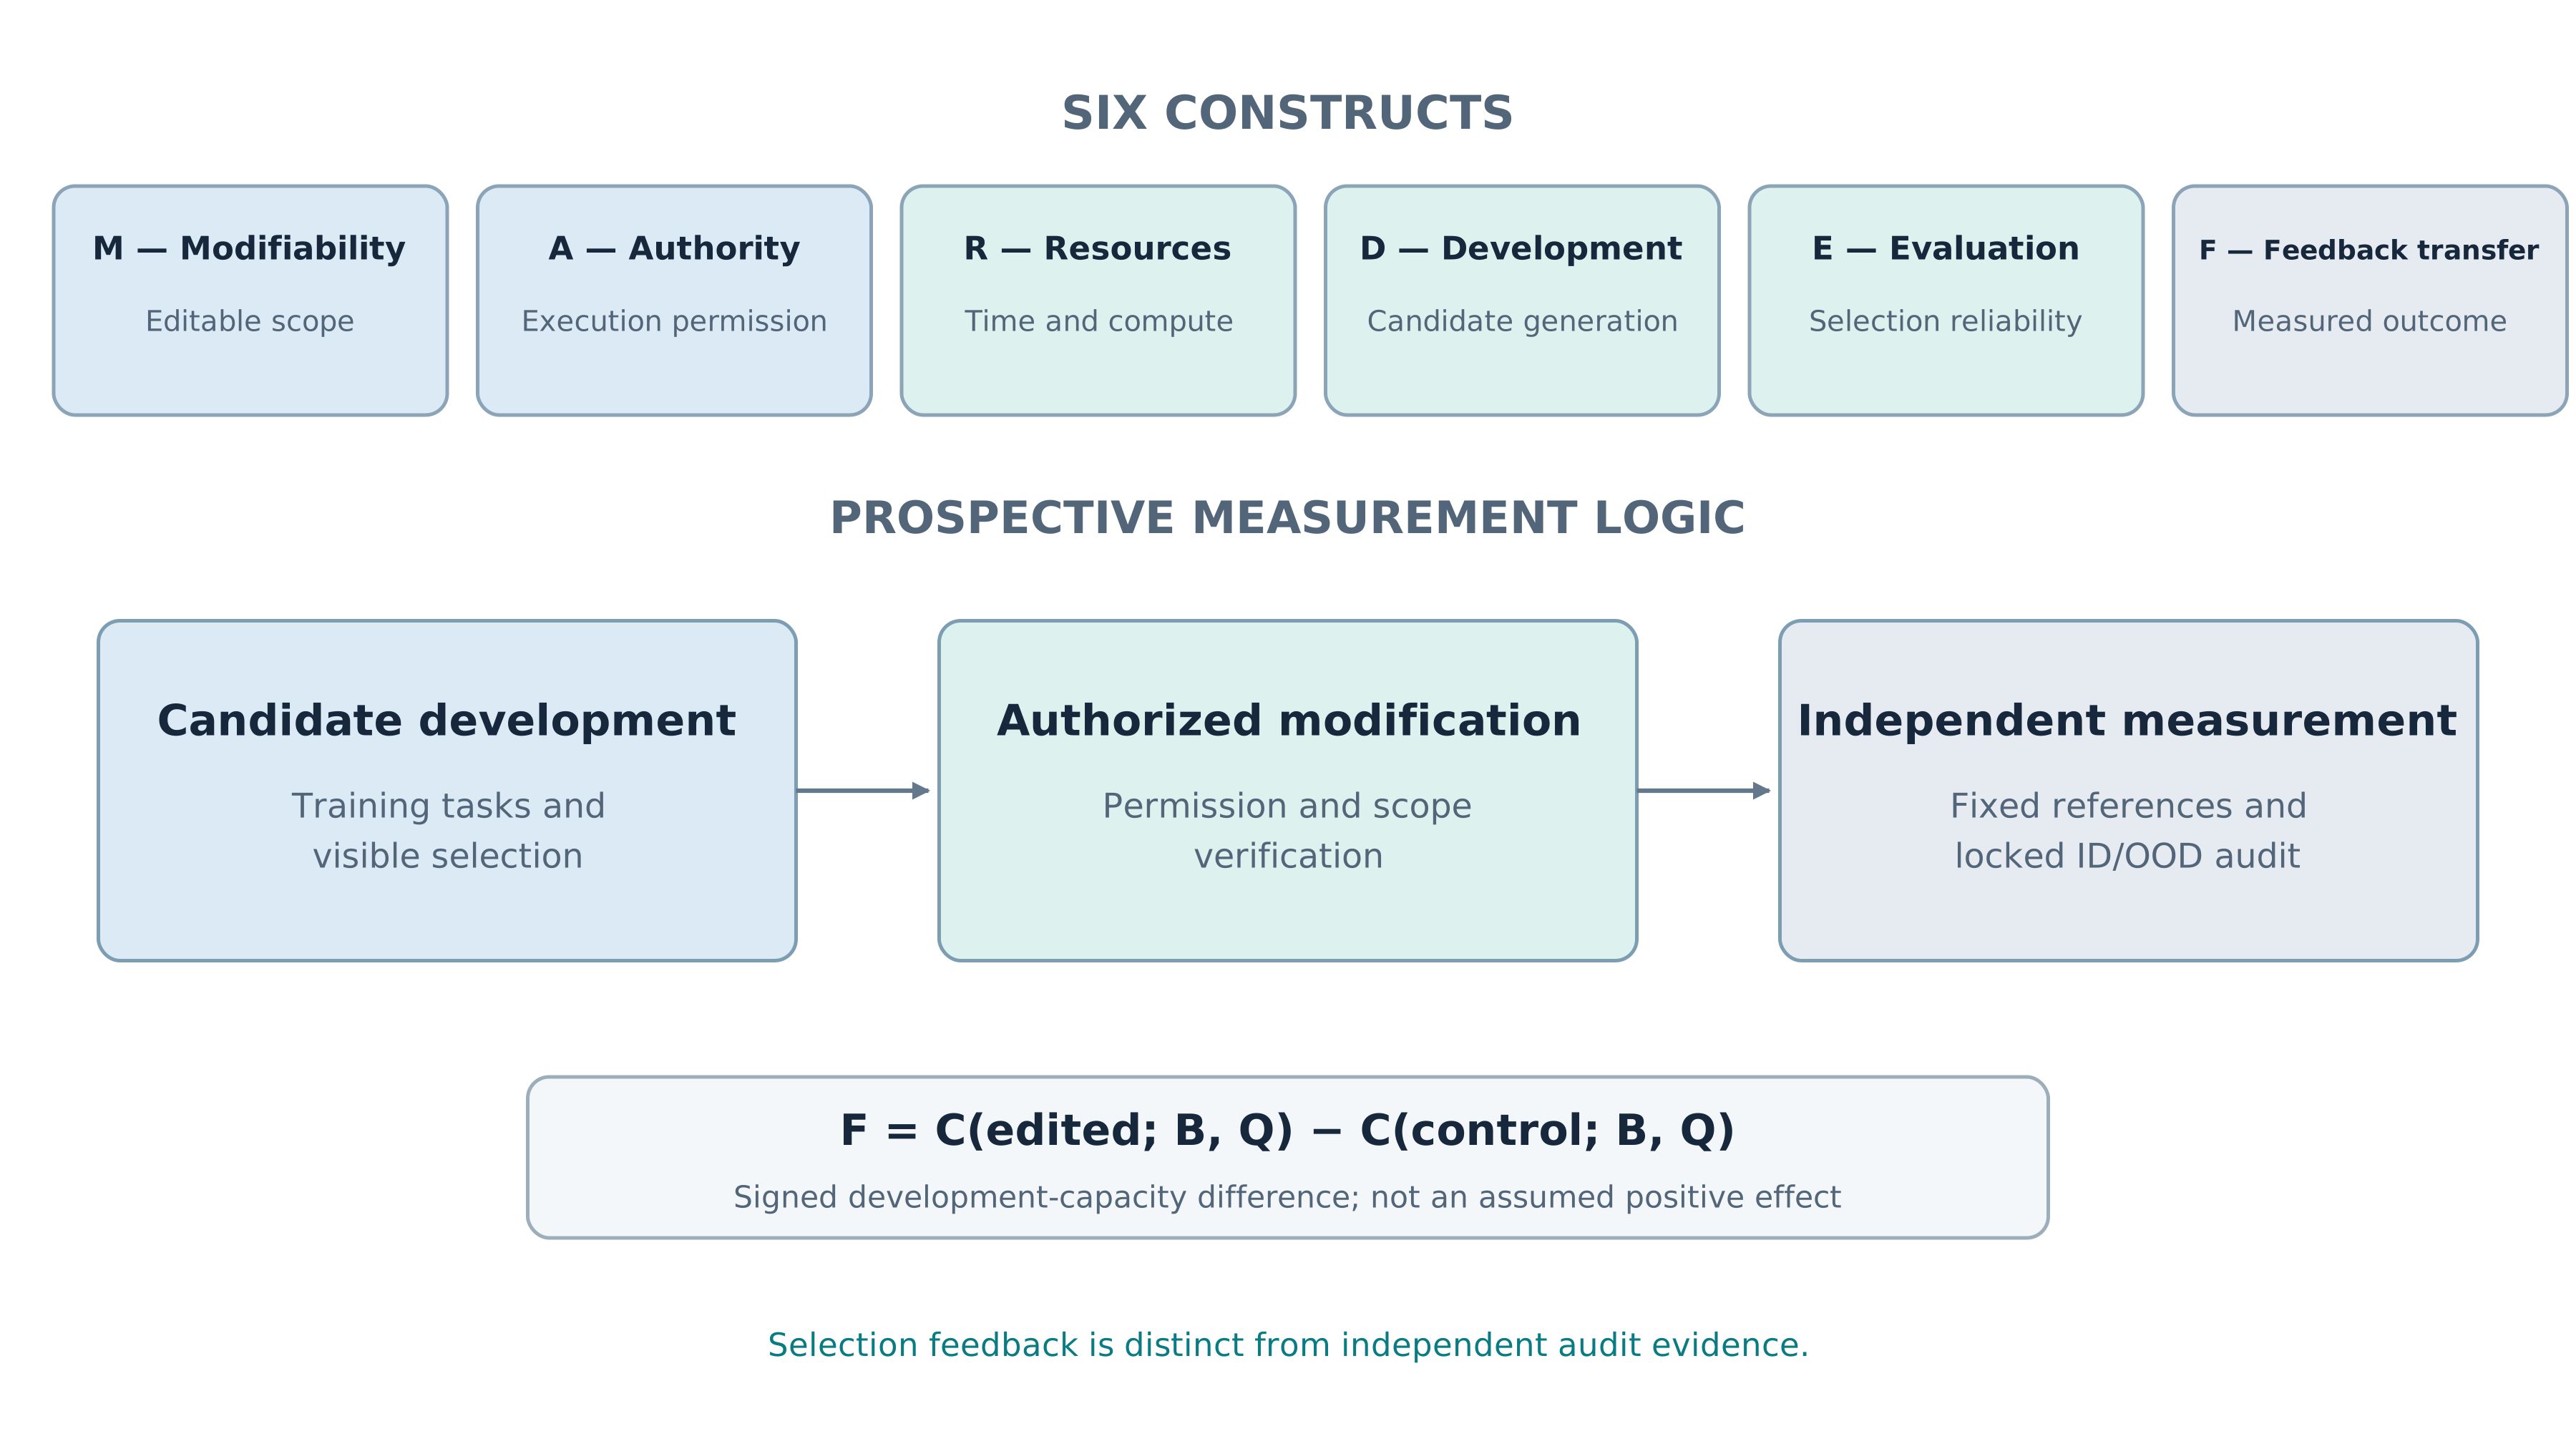
\includegraphics[width=\linewidth]{SMCEP_Figure_2_clean.png}
    \caption{Six SMCEP constructs and their roles in the
    proposed measurement framework. Feedback transfer
    ($F$) is an independently measured, signed
    development-capacity outcome.}
    \label{fig:smcep-six-constructs}
\end{figure}

The operationalization of evaluation reliability $E$ can draw upon structured agent-evaluation taxonomies. Mohammadi et al.\ organize agent assessment along evaluation objectives (behavior, capabilities, reliability, safety) and evaluation processes (interaction modes, datasets, metrics, contexts) \cite{mohammadi2025evaluation}. Because stochastic agent outcomes depend on the execution
trajectory, different repeated-trial metrics answer different reliability questions. We distinguish
$\mathrm{pass}@k$, the probability that at least one of $k$ attempts succeeds, from $\mathrm{pass}^k$, defined here as the probability that all $k$ attempts succeed under a prespecified repeated-trial protocol. These metrics characterize different aspects of task-level success and consistency; neither alone identifies development capacity. The broader need for multidimensional agent evaluation is discussed by Mohammadi et al.\ \cite{mohammadi2025evaluation}. Independent out-of-distribution probes and repeated runs are needed to characterize generalization and uncertainty.

We do not assume these constructs are independent, sufficient, or jointly monotonic. In particular, \(F\) is an outcome of an intervention, not a positive coefficient inserted into the transition equation. Treating \(F\) as a predetermined multiplier of performance gain would presuppose the conclusion. A system may have broad edit permissions yet poor evaluative feedback, or high task competence yet weak transferable development capability.

\subsection{Operational mapping of the six constructs}

The six SMCEP constructs do not constitute six
interchangeable scalar variables. They specify
different components of a development experiment:
intervention scope, authorization, measurement
conditions, resources, proposal mechanisms, and
counterfactual outcomes.

Let $\mathcal{U}(M)$ denote the set of modifications
permitted by the technical edit scope $M$.
Let $a_A(u,h)\in\{0,1\}$ indicate whether a proposed
modification $u$ is authorized under authority
configuration $A$ and the relevant execution
history $h$. The set of technically editable
components need not coincide with the set of
modifications authorized for execution or deployment.

Let $\pi_D(u\mid X,q,h;R)$ denote the
candidate-proposal distribution associated with
development mechanism $D$, current system state
$X$, development task $q$, history $h$, and
resource policy $R$. A candidate can be proposed
only within the specified technical interface,
and its execution remains subject to $a_A$.
The proposal distribution characterizes how
candidate modifications are generated; it is
not itself a measurement of their realized
development benefit.

Evaluation reliability $E$ characterizes the
selection-feedback process, including noise,
calibration, contamination, and dependence on
previous evaluations. Denote the visible
selection signal by
\[
\widetilde{s}_{E}(u,q,h).
\]
This signal may influence candidate selection, but must remain distinct from the locked independent-audit score. The reliability of the latter must be documented separately; independence alone does not guarantee that an audit is valid or sufficiently precise.

Under a specified configuration $\theta=(M,A,E,R,D)$, a development procedure generates, screens, and selects a candidate using only authorized operations and permitted feedback. Its realized development capacity is assessed using the fixed-reference, selected-candidate independent-audit protocol defined in Appendix~B.

Finally, feedback transfer $F$ is defined through a counterfactual comparison of subsequent development capacities, as in Eq.~\eqref{eq:feedback}. It is not an input coefficient in $\theta$, and its sign is not assumed in advance.

This mapping does not assert that the five design components are statistically independent or that their effects are additive. Interactions among modification scope, authorization, evaluation reliability, resources, and proposal competence are empirical questions. In particular, changes
in $M$ or $A$ may alter which development policies can be realized, while changes in $E$ or $R$ may alter candidate selection without improving the underlying proposal mechanism.

For reproducibility, each experimental condition should specify the editable artifacts and operators, authorization gates, proposal and selection procedures, evaluation partitions, resource policies, and the counterfactual comparison used to estimate $F$.

\subsection{Operational boundaries of modifiability and authority}
The distinction between $M$ and $A$ is operational rather than merely terminological. $M$ specifies the \emph{type and location} of a proposed intervention; $A$ specifies whether, by whom, and under what conditions that intervention may be applied. Neither is necessarily a single numerical coefficient. In particular, the ability to \emph{propose} a code or prompt edit does not establish permission to execute it, deploy it, or change the rules that authorize future edits. Table~\ref{tab:scopeauthority} illustrates this distinction; the examples specify possible configurations, not observed capabilities of any named model.
\begin{table}[htbp]\centering\small
\begin{tabularx}{\linewidth}{@{}p{0.21\linewidth}X X@{}}\toprule
Editable scope ($M$) & Possible authority boundary ($A$) & What the resulting observation establishes \\\midrule
Prompt or agent instruction & Agent may propose a revision; human or external controller must approve activation & Proposal capability, not autonomous deployment authority \\
Tool configuration or skill repository & Agent may edit within a sandbox; production promotion requires independent review & Bounded execution authority, not permission to modify oversight \\
Repository source code & Agent may patch and run tests in an isolated branch; merge and release are separately gated & Code-edit and test competence, not unrestricted production control \\
Model weights or training procedure & Weight updates require a separately provisioned training pipeline, compute, and authorization & A different intervention class requiring its own audit and causal design \\\bottomrule
\end{tabularx}
\caption{Illustrative modification scopes and authorization gates. Actual $M$ and $A$ must be specified for each experiment, including permissions to propose, execute, persist, and deploy edits.}\label{tab:scopeauthority}
\end{table}
For example, an agent that generates a plausible patch but cannot execute it without approval has nonempty proposal scope under $M$, yet lacks unilateral deployment authority under $A$. Calling its entire authority ``zero'' would conceal the distinction between sandbox execution, review, and production deployment. Conversely, permission to modify weights does not imply the computational resources $R$, development competence $D$, or reliable feedback $E$ needed for a useful update. A reproducible experiment should report the editable artifact, allowed edit operator, execution environment, approval gate, persistence rule, and rollback procedure. These are design coordinates for $M$ and $A$, not an assumed monotonic ladder from prompts to weights.

The role of the system in its own development process requires similar specification. An agent may function primarily as an instrument within a development process designed and controlled by external actors, or it may participate in determining how subsequent development is conducted. Code access alone does not capture this difference. What matters is the extent to which the system can examine its development procedure, generate and select modifications to that procedure, execute authorized changes, and evaluate their consequences through independent feedback. In SMCEP, these capabilities are represented through the interaction of $M$, $A$, $D$, $E$, and $R$, without introducing an additional autonomy variable. The distinction is therefore operational, not a new claim about agency or consciousness.

\section{Mathematical Formulation and Operational Definitions}
\subsection{Task performance and development capacity}
For a task distribution $\mathcal{T}_P$ and a bounded scoring rule $s$, define
\begin{equation}
P(X_t;\mathcal{T}_P)=\mathbb{E}_{z\sim\mathcal{T}_P}[s(X_t,z)].\label{eq:performance}
\end{equation}
To characterize future development competence, fix a development-task distribution $\mathcal{Q}$, candidate budget $B$, and a prespecified net-gain functional $G_{\mathrm{net}}$ that accounts for failures and relevant costs. The following expression is a general conceptual estimand, not a claim that all historical pilots implemented an identical capacity metric. For prospective real-LLM experiments, the primary operational endpoint is the independently audited gain of the candidate selected without access to audit outcomes, as specified in Eq.~\eqref{eq:realanchor}. Cost-adjusted capacity is defined separately in Eq.~\eqref{eq:netcapacity}.
\begin{equation}
C(X_t;B,\mathcal{Q})=\mathbb{E}_{q\sim\mathcal{Q},\,\xi}\left[G_{\mathrm{net}}(X_t,q,B,\xi)\right].\label{eq:capacity}
\end{equation}
The proposal-policy component of $X_t$ may be evaluated on a common collection of fixed external starting states $Y_j^0$, rather than on the changing $X_t$ itself. This \emph{anchor} construction reduces, but does not eliminate, the confounding effect of shrinking improvement headroom:
\begin{equation}
C_{\mathrm{anchor}}(X_t;B)=\mathbb{E}_{j,\xi}\left[\max_{1\leq k\leq B}\{s(Y_j^0+\delta_k(\pi_t,\xi),q_j)-s(Y_j^0,q_j)\}\right].\label{eq:anchor}
\end{equation}
Here $\pi_t$ is the candidate-generation policy and $\delta_k$ denotes a proposed modification to a fixed reference system. The notation $Y_j^0+\delta_k$ denotes application of an edit rather than
necessarily arithmetic addition.

For prospective experiments, the reference set should include prespecified strata of initial
system competence and modification difficulty, rather than relying exclusively on a single
weak starting state. Let $\mathcal{Q}_h$ denote the development-task distribution associated with reference stratum $h$. Capacity may then be reported separately as $C_{\mathrm{audit}}^{\mathrm{gross}}
(X;B,\mathcal{Q}_h)$ for each stratum, with any aggregate defined using fixed, preregistered stratum weights.

This stratification helps distinguish genuine changes in development competence from changes
in available improvement headroom. It does not eliminate all reference-selection bias,
and the reference panels, weights, and evaluation conditions must remain identical
across experimental arms.

Equation~\eqref{eq:anchor} is an idealized oracle best-of-$B$ opportunity measure. Because its maximum is computed using the evaluation scores of all proposed candidates, it must not be interpreted as the independently audited performance of a candidate selected by the developer without access to those scores. Its value also depends on the candidate budget, the reference-state distribution, and the
evaluation procedure. Conceptual Equation~\eqref{eq:anchor} permits negative gains when all proposed edits are detrimental, whereas pilot v0.8 used a clipped proxy. Retaining negative gains avoids the
nonnegativity imposed by clipping but does not, by itself, guarantee unbiased causal identification. To reduce headroom confounding, v1.0 uses fixed-reference development probes and evaluates development-selected candidates on separate audit tasks, retaining negative gains. The stronger prospective selection--audit firewall, including restrictions on adaptive audit reuse, is specified in Section~\ref{sec:firewall} and Appendix~B.

The historical v0.8 fixed-anchor probe uses a clipped best-of-$B$ opportunity measure, which is nonnegative by construction. Equation~\eqref{eq:anchor}, in contrast, defines an unclipped oracle measure and can take negative values when all proposed edits are detrimental.

Versions v0.9 and v1.0 instead select a candidate using development-task feedback and evaluate that selected candidate on separate audit tasks, retaining negative audit gains.

These historical measures are not numerically interchangeable. The prospective real-LLM protocol therefore prioritizes the selected-candidate independent-audit estimand in Eq.~\eqref{eq:realanchor}, while retaining the oracle measure as a diagnostic of candidate-generation opportunity rather
than realized development capacity.

A further distinction concerns the no-edit option. Equation~\eqref{eq:anchor} maximizes over the
$B$ proposed edits and does not explicitly include a no-op candidate. Consequently, its value can be
negative if all proposed edits reduce performance.

If an unchanged reference is included as an additional candidate, the corresponding oracle opportunity score becomes
\[
C_{\mathrm{anchor}}^{+0}(X_t;B)
=
\mathbb{E}_{j,\xi}
\left[
\max\left\{
0,\,
\max_{1\leq k\leq B}
\left[
s(Y_j^0+\delta_k(\pi_t,\xi),q_j)
-
s(Y_j^0,q_j)
\right]
\right\}
\right].
\]

This quantity is nonnegative by construction, but it still assumes oracle access to the candidate evaluation scores. It must not be confused with the selected-candidate audit estimand in Eq.~\eqref{eq:realanchor}, where the no-edit decision is made without access to the locked audit outcomes. A zero gain under that protocol may reflect a no-edit decision rather than successful development.

Neither historical implementation fully realizes the cost-adjusted general estimand in Eq.~\eqref{eq:capacity}. The prospective real-LLM protocol in Appendix~B specifies additional failure, resource-accounting, and audit-isolation requirements.

A held-out set of ordinary coding questions measures generalization of task performance $P$; it does not, by itself, measure second-order development capacity $C$. To operationalize $C$ in a real LLM agent, the development agent proposes bounded edits to independently initialized reference agents or software artifacts. These edits are then executed and scored against reference baselines on independent tasks under equal candidate budgets. The fixed reference controls for headroom, while separate ID and OOD development-task families probe transfer. The audit-only dataset remains strictly unavailable to the candidate selector, even through aggregate score feedback.\par

The separation between immediate task performance $P(X_t)$ and second-order development capacity $C(X_t)$ has an empirical analogue in software-engineering benchmarks. Traditional benchmarks predominantly measure short-horizon bug fixes, such as single-issue commits averaging roughly 33 lines of code in SWE-bench Verified, where frontier models already exceed 80\% \cite{xu2026roadmapbench}. Real-world self-modification, by contrast, requires multi-target, long-horizon software engineering. ROADMAPBENCH operationalizes this setting with 115 version-upgrade tasks across 17 repositories and 5 programming languages, where the median oracle patch modifies approximately 3,700 lines across 51 files and a median of 5 subtasks \cite{xu2026roadmapbench}. In the reported single-trial evaluation under the
OpenHands scaffold, Claude-Opus-4.7 achieves the highest resolved rate (39.1\%), while the lowest reported rate is 5.2\% \cite{xu2026roadmapbench}. These are benchmark-specific outcomes rather than
estimates of general software-development competence. This contrast motivates studying development ability on multi-component tasks, but ROADMAPBENCH success rates are not direct measurements of the SMCEP fixed-anchor capacity estimand $C_{\mathrm{anchor}}$. These results are cited as external motivating evidence, not as measurements from the present simulator.

\subsection{Counterfactual feedback transfer}
For an eligible modification $u_t$, define two matched intervention branches originating from the same state $X_t$:
\begin{align}
X_{t+1}^{(1)}
&=\operatorname{Transition}(X_t,u_t,\omega_t),\\
X_{t+1}^{(0)}
&=\operatorname{Transition}(X_t,\varnothing,\omega_t),\\
F_t(u_t;B,\mathcal{Q})
&=C(X_{t+1}^{(1)};B,\mathcal{Q})
-C(X_{t+1}^{(0)};B,\mathcal{Q}).
\label{eq:feedback}
\end{align}
Here $\varnothing$ denotes withholding the candidate modification while preserving the specified control
procedure, and $\omega_t$ represents matched exogenous conditions where these can be controlled.
The contrast isolates the modification only insofar as other relevant interventions, resources, and
evaluation conditions are held comparable.
Where feasible, the two branches should share development tasks, evaluation budgets, and random-number streams. This contrast is a controlled potential-outcome comparison, not automatically an identified causal effect in an observational agent log. Selecting $u_t$ based on observed performance can induce bias; prospective randomization or a fully specified intervention protocol mitigates this risk. $F_t>0$ on a single probe is not sufficient to establish durable recursion. Likewise,
\begin{equation}
\Delta P_t>0\;\not\!\implies\;\Delta C_t>0.
\end{equation}
A sustained recursive-improvement claim would require pre-specified evidence of transferable positive development-capacity effects over multiple generations and relevant task distributions, with uncertainty and counterfactual comparisons. Related reward-tampering and reward-hacking formalisms motivate careful separation of the evaluator from the optimizing agent \cite{everitt2021,skalse2022}; the counterfactual capacity estimand defined here is distinct from those formalisms. No universal numerical transition threshold is assumed.

\subsection{Identification and evaluation separation}
A development loop may use training tasks to propose candidates and a noisy selection evaluator to choose among them. Independent ID and OOD probe sets should not be used in candidate selection. This separation matters because repeated optimization against a score can lead to selection-induced overfitting, without establishing intentional manipulation or an inevitable failure mode \cite{goodhart1984}. Even a nominally held-out set can lose independence if its results repeatedly inform model selection or researcher revisions. Work on test-data reuse for evolving algorithms documents this adaptive-overfitting risk in a different setting \cite{gossmann2021}. We therefore distinguish three non-overlapping partitions: a visible selection set, a development-only validation set, and a locked final audit set. Repeated diagnostic probes may be reported, but should not be described as untouched final holdouts if their outcomes influence design decisions. AIDE2 illustrates a layered agent-improvement workflow \cite{srikanth2026}, but its findings do not independently validate the SMCEP estimand. Evaluation reliability remains an empirical question, not an assumed collapse rule. A rigorous audit combines such separation with multi-trial consistency metrics (e.g., $\mathrm{pass}^k$) and independent out-of-distribution probes \cite{mohammadi2025evaluation}.

\section{Experimental Methodology}
\subsection{Synthetic environment and scope}
The pilot environment is a researcher-defined, low-dimensional nonlinear task landscape. Agent state includes a four-dimensional task parameter vector and, in editable-policy conditions, a small proposal-policy parameterization (including step-size and bias). Candidate proposals are generated and selected using noisy task feedback. Independent probes evaluate task performance and, in later versions, development-policy behavior on fixed reference states. These are synthetic agents, not deployed language-model research agents, and the simulator's search operators do not approximate the full engineering complexity of code-based recursive self-improvement.

\subsection{Real-LLM feasibility experiments (T0--T7): design and evidence boundaries}\label{sec:real-llm-methods}
A separate series of exploratory experiments used open-weight language models in bounded coding and development-policy workflows. T0 established baseline behavior; T1--T3 examined paired frozen/evolving outputs, error feedback, and transfer-related evaluation problems. T4--T5 ran three development--selection--locked-audit cycles each, with candidate procedures evaluated against the incumbent. T6 compared frozen, linear, and hybrid archive-assisted development conditions in a ten-turn pilot. T7 comprised real-model task-bank calibration followed by a distinct stochastic mechanism simulation. The latter is \emph{not} a 50-generation real-LLM recursive-improvement run. Model calls, candidate edits, test executions, and audit decisions must be distinguished from independently replicated experimental units. These feasibility studies do not instantiate the full cost-adjusted, preregistered causal protocol defined in Appendices B--C.



\subsection{Successive pilot designs}
\begin{table}[htbp]\centering\small
\begin{tabularx}{\linewidth}{@{}l l X@{}}\toprule
Version & Design emphasis & Primary methodological issue \\\midrule
v0.6 & Static, restricted, broad, noisy selection & Initial $P$--$C$ separation; capacity/headroom confounding \\
v0.7 & Six-group scope and policy ablations & Development-policy editability; remaining-headroom dependence \\
v0.8 & Fixed-reference anchor probes & Separation of policy competence from current-agent headroom \\
v0.9 & Independent ID and OOD anchors & Transfer across synthetic task distributions \\
v1.0 & Paired frozen-policy versus evolving-policy arms & Multi-generation contrast under matched initial seeds \\\bottomrule
\end{tabularx}\caption{Exploratory methodological progression. Versions are not independent replications and should not be pooled as if they were.}\label{tab:design}
\end{table}

The v0.6 pilot used 12 seeds, 20 generations, and eight candidates per generation. Later pilots used 12 seeds, 25 generations, and six candidates per generation. Version-specific probe counts and randomization rules are documented in the accompanying scripts and JSON outputs. Version changes modified the estimand and sometimes the experimental implementation; numerical values are therefore not directly comparable across all five pilots.

\subsection{Synthetic transition and selection rules}

The v1.0 simulator represents each agent by $X_t=(\theta_t,\ell_t,b_t)$, where $\theta_t\in[-2,2]^4$ is the task-parameter vector, $\ell_t$ is the logarithmic proposal step size, and $b_t$ is a scalar proposal bias. Both experimental arms begin from the same initial state.

For each of $B=6$ candidates, the simulator samples $z_k\sim\mathcal{N}(0,I_4)$ and proposes
\[
\theta_{t,k}'=
\operatorname{clip}_{[-2,2]}
\left[
\theta_t+\exp(\ell_t)(z_k+b_t\mathbf{1})
\right].
\]

In the frozen-policy arm, $\ell_t$ and $b_t$ remain unchanged. In the evolving-policy arm, candidates additionally contain
\[
\ell_{t,k}'=
\operatorname{clip}
\left(\ell_t+\epsilon_{\ell,k},
\log 0.04,\log 1.2\right),
\]
\[
b_{t,k}'=
\operatorname{clip}
\left(b_t+\epsilon_{b,k},-1.2,1.2\right),
\]
where
$\epsilon_{\ell,k}\sim\mathcal{N}(0,0.18^2)$
and
$\epsilon_{b,k}\sim\mathcal{N}(0,0.12^2)$.

Candidate selection combines task-score improvement and a development-policy probe difference:
\[
U_{t,k}=
\Delta P_{t,k}^{\mathrm{sel}}
+
w\left(
C_{t,k}^{\mathrm{sel}}
-
C_t^{\mathrm{sel}}
\right),
\qquad w=1.
\]

The observed selection utility is
\[
\widetilde U_{t,k}
=
U_{t,k}+\eta_{t,k},
\qquad
\eta_{t,k}\sim\mathcal{N}(0,0.015^2).
\]

The candidate with the largest observed utility is accepted only if that utility is positive; otherwise the state remains unchanged. Selection-policy probes are distinct from the reported fixed-reference ID and OOD audits.

The synthetic task score is computed from a bounded nonlinear function of weighted squared distance and sinusoidal variation. The exact task-generation distributions, score implementation, deterministic
random-stream construction, and probe sample sizes are specified in the versioned simulation source code.

These rules describe the implemented synthetic experiment, not a general transition law for autonomous AI systems.

\subsection{Paired estimand for v1.0}
The latest experiment compares two conditions in which task-parameter edits are available in both arms.
The \emph{frozen-policy} arm generates candidates without policy-parameter mutations, whereas the
\emph{evolving-policy} arm additionally permits mutations of the proposal-policy parameters.

The intervention therefore changes the admissible candidate space as well as the possibility of
development-policy adaptation. The resulting contrast estimates the effect of this bundled intervention
within the specified simulator, rather than the isolated effect of policy learning independent of
candidate-space differences. For endpoint $Y\in\{P,C_{\id},C_{\ood}\}$, define
\begin{equation}
\widehat\tau_Y=\frac{1}{N}\sum_{s=1}^{N}\left[(Y^{\mathrm{evolving}}_{T,s}-Y^{\mathrm{evolving}}_{0,s})-(Y^{\mathrm{frozen}}_{T,s}-Y^{\mathrm{frozen}}_{0,s})\right],\label{eq:paired}
\end{equation} with $N=12$ matched seeds and $T=25$ generations. Because both arms are initialized with matched seeds and follow explicitly specified intervention rules, the paired contrast describes the effect of the implemented arm assignment within this deterministic simulation protocol. Matching seeds reduces variation from initial conditions and shared random streams, but does not remove differences introduced by the arm-specific candidate-generation rules. The contrast is therefore interpretable only for this bundled intervention in a researcher-designed environment; it does not identify an isolated effect of policy adaptation or a causal effect in deployed AI systems.
The v1.0 selection objective and test task generation remain researcher-designed; no blinded preregistration was performed. The simulator's generation count and proposal budget are not directly comparable with human-equivalent task durations in METR time-horizon evaluations \cite{metr2025measuring,metr2026timehorizon}. The present results remain exploratory because of the synthetic task design and limited statistical and external validation.

\subsection{Methodological role of the synthetic pilots}
The synthetic pilots serve as a methodological proof of concept for distinguishing task performance from future development capacity. Their successive designs expose measurement trade-offs involving improvement headroom, fixed-reference probes, and development-policy editability. The resulting observations are exploratory and motivate the independent-audit and causal protocols specified in
Section~\ref{sec:validationprotocol} and Appendices B--C.

\section{Exploratory Results}
\subsection{Progression across pilot versions}
\begin{table}[htbp]\centering\small
\begin{tabular}{@{}llrrl@{}}\toprule
Version & Condition & $\overline{\Delta P}$ & $\overline{\Delta C}$ & Capacity metric \\\midrule
v0.6 & Restricted (B) & $+0.0425$ & $-0.0264$ & Self-referential probe \\
v0.6 & Broad (C) & $-0.0892$ & $-0.0432$ & Self-referential probe \\
v0.7 & Broad + policy (C) & $+0.0637$ & $-0.0327$ & Self-referential probe \\
v0.7 & Noisy broad (D) & $-0.1523$ & $-0.0021$ & Self-referential probe \\
v0.8 & Broad + policy (C) & $+0.0601$ & $-0.0088$ & Fixed anchor \\
v0.8 & Noisy broad (D) & $-0.1194$ & $-0.0145$ & Fixed anchor \\
v0.9 & Broad + policy (C) & $+0.0666$ & $-0.0278$ & OOD fixed anchor \\
v0.9 & Noisy broad (D) & $-0.0538$ & $-0.0191$ & OOD fixed anchor \\\bottomrule
\end{tabular}\caption{Selected descriptive outcomes from archived pilot summaries. Metric definitions differ by version; this table illustrates methodological evolution, not a single controlled comparison.}\label{tab:progression}
\end{table}

\paragraph{Limits of cross-version comparability.}

Table~\ref{tab:progression} reports selected historical outcomes from experiments with different operational definitions, intervention conditions, and evaluation procedures. Consequently, differences between versions must not be interpreted as improvements or declines on a common development-capacity
scale.

In v0.6 and v0.7, capacity probes were self-referential and remained sensitive to the current system state and available improvement headroom. Version v0.8 introduced fixed-reference opportunity probes, while v0.9 evaluated selected candidates on separate ID and OOD reference tasks. These changes alter
the estimand rather than merely improving the precision of an unchanged measurement.

The condition labels B, C, and D are version-specific experimental identifiers. Their reuse does not establish identical interventions, resource allocations, or evaluation conditions across versions.
Accordingly, the table supports a methodological comparison of successive pilot designs, not a pooled statistical analysis or a causal comparison across versions.

The v1.0 paired experiment is reported separately in Table~\ref{tab:v10}. Its matched-seed comparison is meaningful within that version's specified protocol, but it does not retroactively place the
earlier pilot outcomes on a common scale.

In several pilots, we observed improvements in task performance alongside declines in the corresponding
development-capacity measure. This divergence led us to revise the measurement design across successive
versions, particularly by introducing fixed-reference probes. We interpret these results as evidence of a measurement challenge within the simulator, not as a general law governing recursive self-improvement.

\subsection{Paired frozen--evolving comparison (v1.0)}
\begin{table}[htbp]\centering
\begin{tabular}{@{}lrrr@{}}\toprule
Arm & $\overline{\Delta P}$ & $\overline{\Delta C_{\id}}$ & $\overline{\Delta C_{\ood}}$ \\\midrule
Frozen policy & $+0.0730$ & $0.0000$ & $0.0000$ \\
Evolving policy & $+0.0666$ & $-0.0071$ & $-0.0278$ \\
Evolving minus frozen & $-0.0064$ & $-0.0071$ & $-0.0278$ \\\bottomrule
\end{tabular}\caption{Mean end-minus-start changes for 12 paired seeds over 25 generations (v1.0).}\label{tab:v10}
\end{table}

The zero changes in both frozen-policy capacity measures are structural consequences of the implemented probe. The probe evaluates the development-policy parameters against fixed reference states, while the frozen arm holds those policy parameters constant. Thus, task-level improvements in the frozen arm cannot change its measured capacity under this operationalization. These zeros should not be interpreted as independent empirical evidence that frozen development policies have no capacity for improvement under other definitions. Corresponding differences were $-0.0071$ for
ID capacity (descriptive 95\% Student-$t$ interval $[-0.0131,-0.0011]$) and $-0.0278$
for OOD capacity (interval $[-0.0525,-0.0030]$). These intervals use the sample standard deviation of the 12 seed-level paired contrasts and $t_{0.975,11}$ rather than a normal critical value. They remain exploratory, with a small seed count, no multiplicity correction, and no preregistration; they must not be presented as confirmatory tests. Mean acceptance rates were approximately 57.7\% (frozen) and 54.7\% (evolving). Among accepted candidates, 23.1\% in the frozen arm and 29.9\% in the evolving arm had nonpositive latent selection utility, despite positive noisy observed utility.

The simulator records these events as \texttt{false\_accept}. This is a selection-noise diagnostic, not a measure of failure on the independent ID or OOD capacity audits. It should not be interpreted as an empirical rate of unsafe modifications.

For each accepted modification, the simulator also records signed fixed-anchor probe changes
as \texttt{F\_id} and \texttt{F\_ood}. These quantities compare the selected updated state with the preceding state under the same probe seeds and task panels.

In the evolving arm, mean per-accepted-edit changes were approximately $-0.00052$ for ID capacity and $-0.00203$ for OOD capacity. The corresponding values in the frozen arm were structurally zero.

Because the probes use fixed task panels and the modifications are selected adaptively, these quantities are within-simulator diagnostics rather than independently replicated causal effects or evidence of general recursive self-improvement.

The reported descriptive 95\% intervals use the Student-$t$ formulation $\bar d \pm t_{0.975,11}s_d/\sqrt{12}$, where $d$ is the per-seed evolving-minus-frozen endpoint change, $s_d$ is its sample standard deviation, and $t_{0.975,11}\approx 2.201$. The paired design with \(N=12\) matched initial
seeds reduces variability associated with initial conditions and supports an exploratory assessment
of the implemented intervention. However, the limited sample size, simulator-specific design,
and absence of preregistration preclude confirmatory inference or claims of general statistical robustness.

These intervals quantify dispersion across the 12 selected simulator seeds under the specified experimental configuration. They do not incorporate uncertainty about the synthetic environment design, task-family choice, or transfer to real AI systems.

Figure~\ref{fig:v1-results} visualizes the descriptive v1.0 outcomes reported in Table~\ref{tab:v10},
highlighting the distinction between task-performance gains and changes in fixed-reference development capacity.

\paragraph{Structural limitation of the frozen-policy comparison.}

Under the v1.0 fixed-reference capacity operationalization, the frozen arm retains an unchanged development policy throughout the trajectory. Because the capacity probe evaluates this policy on fixed reference states, its measured capacity change is zero by construction, apart from any
measurement variation introduced by the evaluation procedure.

Consequently, the paired capacity-change contrast between the evolving and frozen arms is algebraically equivalent to the evolving arm's capacity change when the frozen-arm change is exactly zero. The frozen arm therefore provides a useful control for task-level improvement under a fixed development policy, but it does not supply an independently varying capacity-change baseline.

The observed negative capacity contrasts should accordingly be interpreted as changes in the evolving policy's audited effectiveness on the specified reference tasks, not as evidence that the frozen
policy causally outperforms every possible alternative development regime.

A stronger causal comparison would require additional intervention arms, such as policy-only updates, matched random policy changes, or controlled modifications of individual policy parameters, with
independent capacity audits across prespecified reference strata.

\paragraph{Alternative explanations of negative capacity transfer.}

The negative ID and OOD capacity changes observed in the evolving-policy arm admit several competing explanations. First, changes in the proposal step size may reduce the effectiveness of the evolved
policy when transferred to fixed reference states with different improvement headroom. A proposal distribution adapted to the current trajectory need not perform well on less-developed reference systems.

Second, allocating a fixed candidate budget across both task-parameter modifications and development-policy modifications may alter the effective search process. Any resulting capacity loss could reflect
resource allocation or candidate-selection effects rather than a general limitation of recursive self-improvement.

Third, policy parameters are selected jointly with task-level candidate changes. A policy modification may therefore be retained because of its association with a favorable task outcome, even when its
independent contribution to future development capacity is neutral or negative. This possibility resembles selection hitchhiking and should not be conflated with demonstrated causal degradation of proposal competence.

The present experiment does not identify the relative contributions of these mechanisms. Distinguishing them would require targeted ablations, including fixed-step-size controls, policy-only
candidate updates, matched search budgets, and capacity probes across multiple reference-state strata.

Accordingly, the negative capacity estimates are evidence about this specific synthetic configuration and measurement protocol, not evidence that recursive self-improvement is generally harmful or impossible.

\begin{figure}[htbp]
\centering
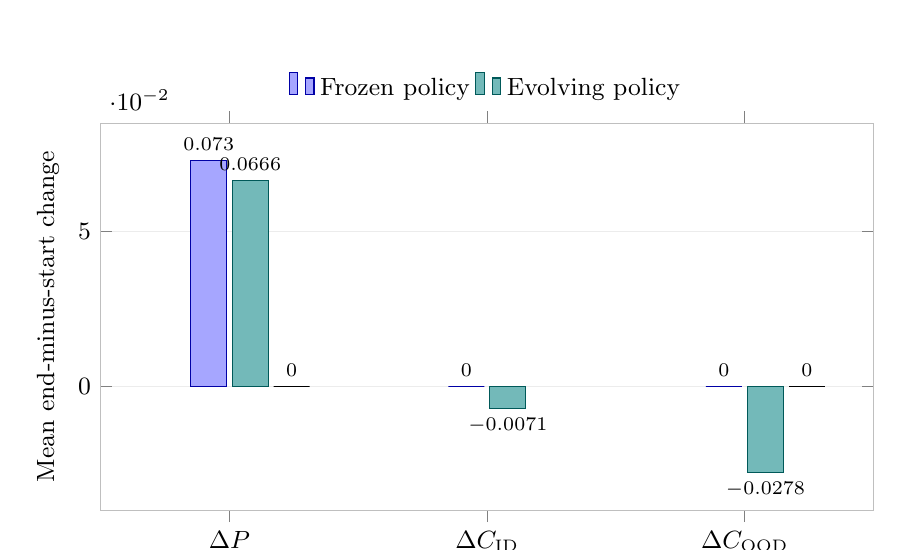
\begin{tikzpicture}
\begin{axis}[
    ybar,
    width=0.94\linewidth,
    height=6.5cm,
    bar width=13pt,
    ymin=-0.04,
    ymax=0.085,
    ylabel={Mean end-minus-start change},
    symbolic x coords={P,ID,OOD},
    xtick=data,
    xticklabels={
        {$\Delta P$},
        {$\Delta C_{\mathrm{ID}}$},
        {$\Delta C_{\mathrm{OOD}}$}
    },
    enlarge x limits=0.25,
    ymajorgrids=true,
    grid style={gray!15},
    axis line style={gray!50},
    tick label style={font=\small},
    label style={font=\small},
    legend style={
        at={(0.5,1.03)},
        anchor=south,
        legend columns=2,
        draw=none,
        font=\small
    },
    nodes near coords,
    every node near coord/.append style={
        font=\scriptsize,
        /pgf/number format/fixed,
        /pgf/number format/precision=4
    },
    nodes near coords align={vertical}
]

\addplot[
    fill=blue!35,
    draw=blue!65!black
] coordinates {
    (P,0.0730)
    (ID,0.0000)
    (OOD,0.0000)
};

\addplot[
    fill=teal!55,
    draw=teal!70!black
] coordinates {
    (P,0.0666)
    (ID,-0.0071)
    (OOD,-0.0278)
};

\legend{Frozen policy,Evolving policy}

\addplot[
    black,
    thin,
    forget plot
] coordinates {
    (P,0)
    (OOD,0)
};

\end{axis}
\end{tikzpicture}

\caption{Descriptive v1.0 results for frozen and
evolving development policies across 12 paired
seeds and 25 generations. Task-performance gains
do not imply positive transfer to fixed-reference
development capacity. Results are exploratory.}

\label{fig:v1-results}
\end{figure}


The evolving policy did not produce positive transfer on the selected held-out ID and OOD probes under this implementation. The OOD tasks use a shifted target distribution and a different landscape frequency, but share the same researcher-defined synthetic task generator and scoring function as the ID tasks. Thus, OOD denotes a specified distribution shift within the simulator, not independent validation across unrelated environments.

We evaluated development capacity on fixed, seed-indexed ID and OOD task panels, allowing matched comparisons across generations without introducing variation from task resampling. Candidate selection and capacity evaluation used disjoint task draws and deterministic seed families. This separation provides a useful within-simulator test of transfer, although both evaluations remain part of the same synthetic task-generating framework.

The fixed panels were reused for diagnostic analysis, rather than refreshed at each generation. We therefore interpret the observed changes as held-out measurements within the simulator, with generalization to new task instances and independently designed environments still requiring prospective evaluation. Such evaluation would also need to prevent repeated audit feedback
from influencing subsequent researcher decisions.

These simulator-level observations are qualitatively consistent with external evidence on task complexity. ROADMAPBENCH reports monotonically decreasing resolved rates as task complexity increases across three structural proxies: files changed, lines changed, and number of targets \cite{xu2026roadmapbench}. The study also analyzes performance by subtask count, illustrating a possible complexity-related bottleneck in the evaluated setup \cite{xu2026roadmapbench}. This parallel is offered as motivating context for the SMCEP distinction between $P$ and $C_{\mathrm{anchor}}$; it is not a measurement from the present pilots and does not establish a causal claim about real AI systems.

\subsection{Why adverse transfer is a central measurement result}
The results in Tables~\ref{tab:progression} and~\ref{tab:v10} illustrate a central measurement distinction: improvements in current task performance need not coincide with improvements in future development capacity. However, the historical pilots use different capacity operationalizations and cannot be treated as independent replications of a common effect. The v1.0 findings describe outcomes within a researcher-defined simulation environment. They do not establish deliberate evaluator
exploitation, a general decline in intelligence, or the causal mechanism responsible for the observed adverse transfer. The negative transfer observed in the evolving-policy arm is not, by itself, evidence of a simulation failure or a general limitation of optimization. Rather, it illustrates how task-performance gains can coexist with adverse changes in a separately operationalized development-capacity measure. This supports the methodological rationale for distinguishing \(P\) from \(C\), without establishing that the present simulator identifies a general failure mechanism in recursive self-improvement.

The result motivates a \emph{prospective} identification question: did a policy update produce a reusable development skill, or did it merely improve selection feedback on the visible tasks? The current pilot does not uniquely identify the mechanism behind the negative transfer. Several explanations remain plausible, including noisy selection, policy parameterization, and differences between task families.

The interaction between evaluation reliability ($E$) and candidate-development capability ($D$)
offers one possible explanation for this divergence. A development policy may become more effective at proposing or selecting changes that perform well under its available evaluation signals without acquiring a correspondingly transferable development skill. If those signals are noisy, incomplete, or insufficiently representative of future tasks, repeated selection can favor locally successful changes that perform poorly under a different evaluation distribution.

This mechanism is consistent with concerns about adaptive overfitting and reward misspecification,
but it has not been causally established by the present simulations. Distinguishing it from candidate-space effects, policy parameterization, and task-family mismatch would require controlled variation in evaluation reliability, matched proposal distributions, and independently generated audit tasks. Such experiments would also clarify whether adverse transfer reflects limitations in candidate development, evaluation, or their interaction.

\subsection{Selection--edit--audit firewall: the prospective test}\label{sec:firewall}
The central proposed safeguard is a separation of \emph{candidate generation}, \emph{selection and authorized execution}, and \emph{independent final audit}. Figure~\ref{fig:firewall} shows the information boundary. A selection evaluator may guide the choice of an edit, but audit labels, item-level scores, and aggregate feedback must not be returned to the development agent or reused for iterative investigator tuning. The selected edit, including a permitted no-edit choice, is evaluated once under prespecified rules on fixed external reference artifacts; unsuccessful attempts remain in the accounting. This procedure addresses the risk of selection-induced overfitting but is \emph{not} itself evidence that overfitting caused the historical v1.0 result.


\begin{figure}[htbp]
    \centering
    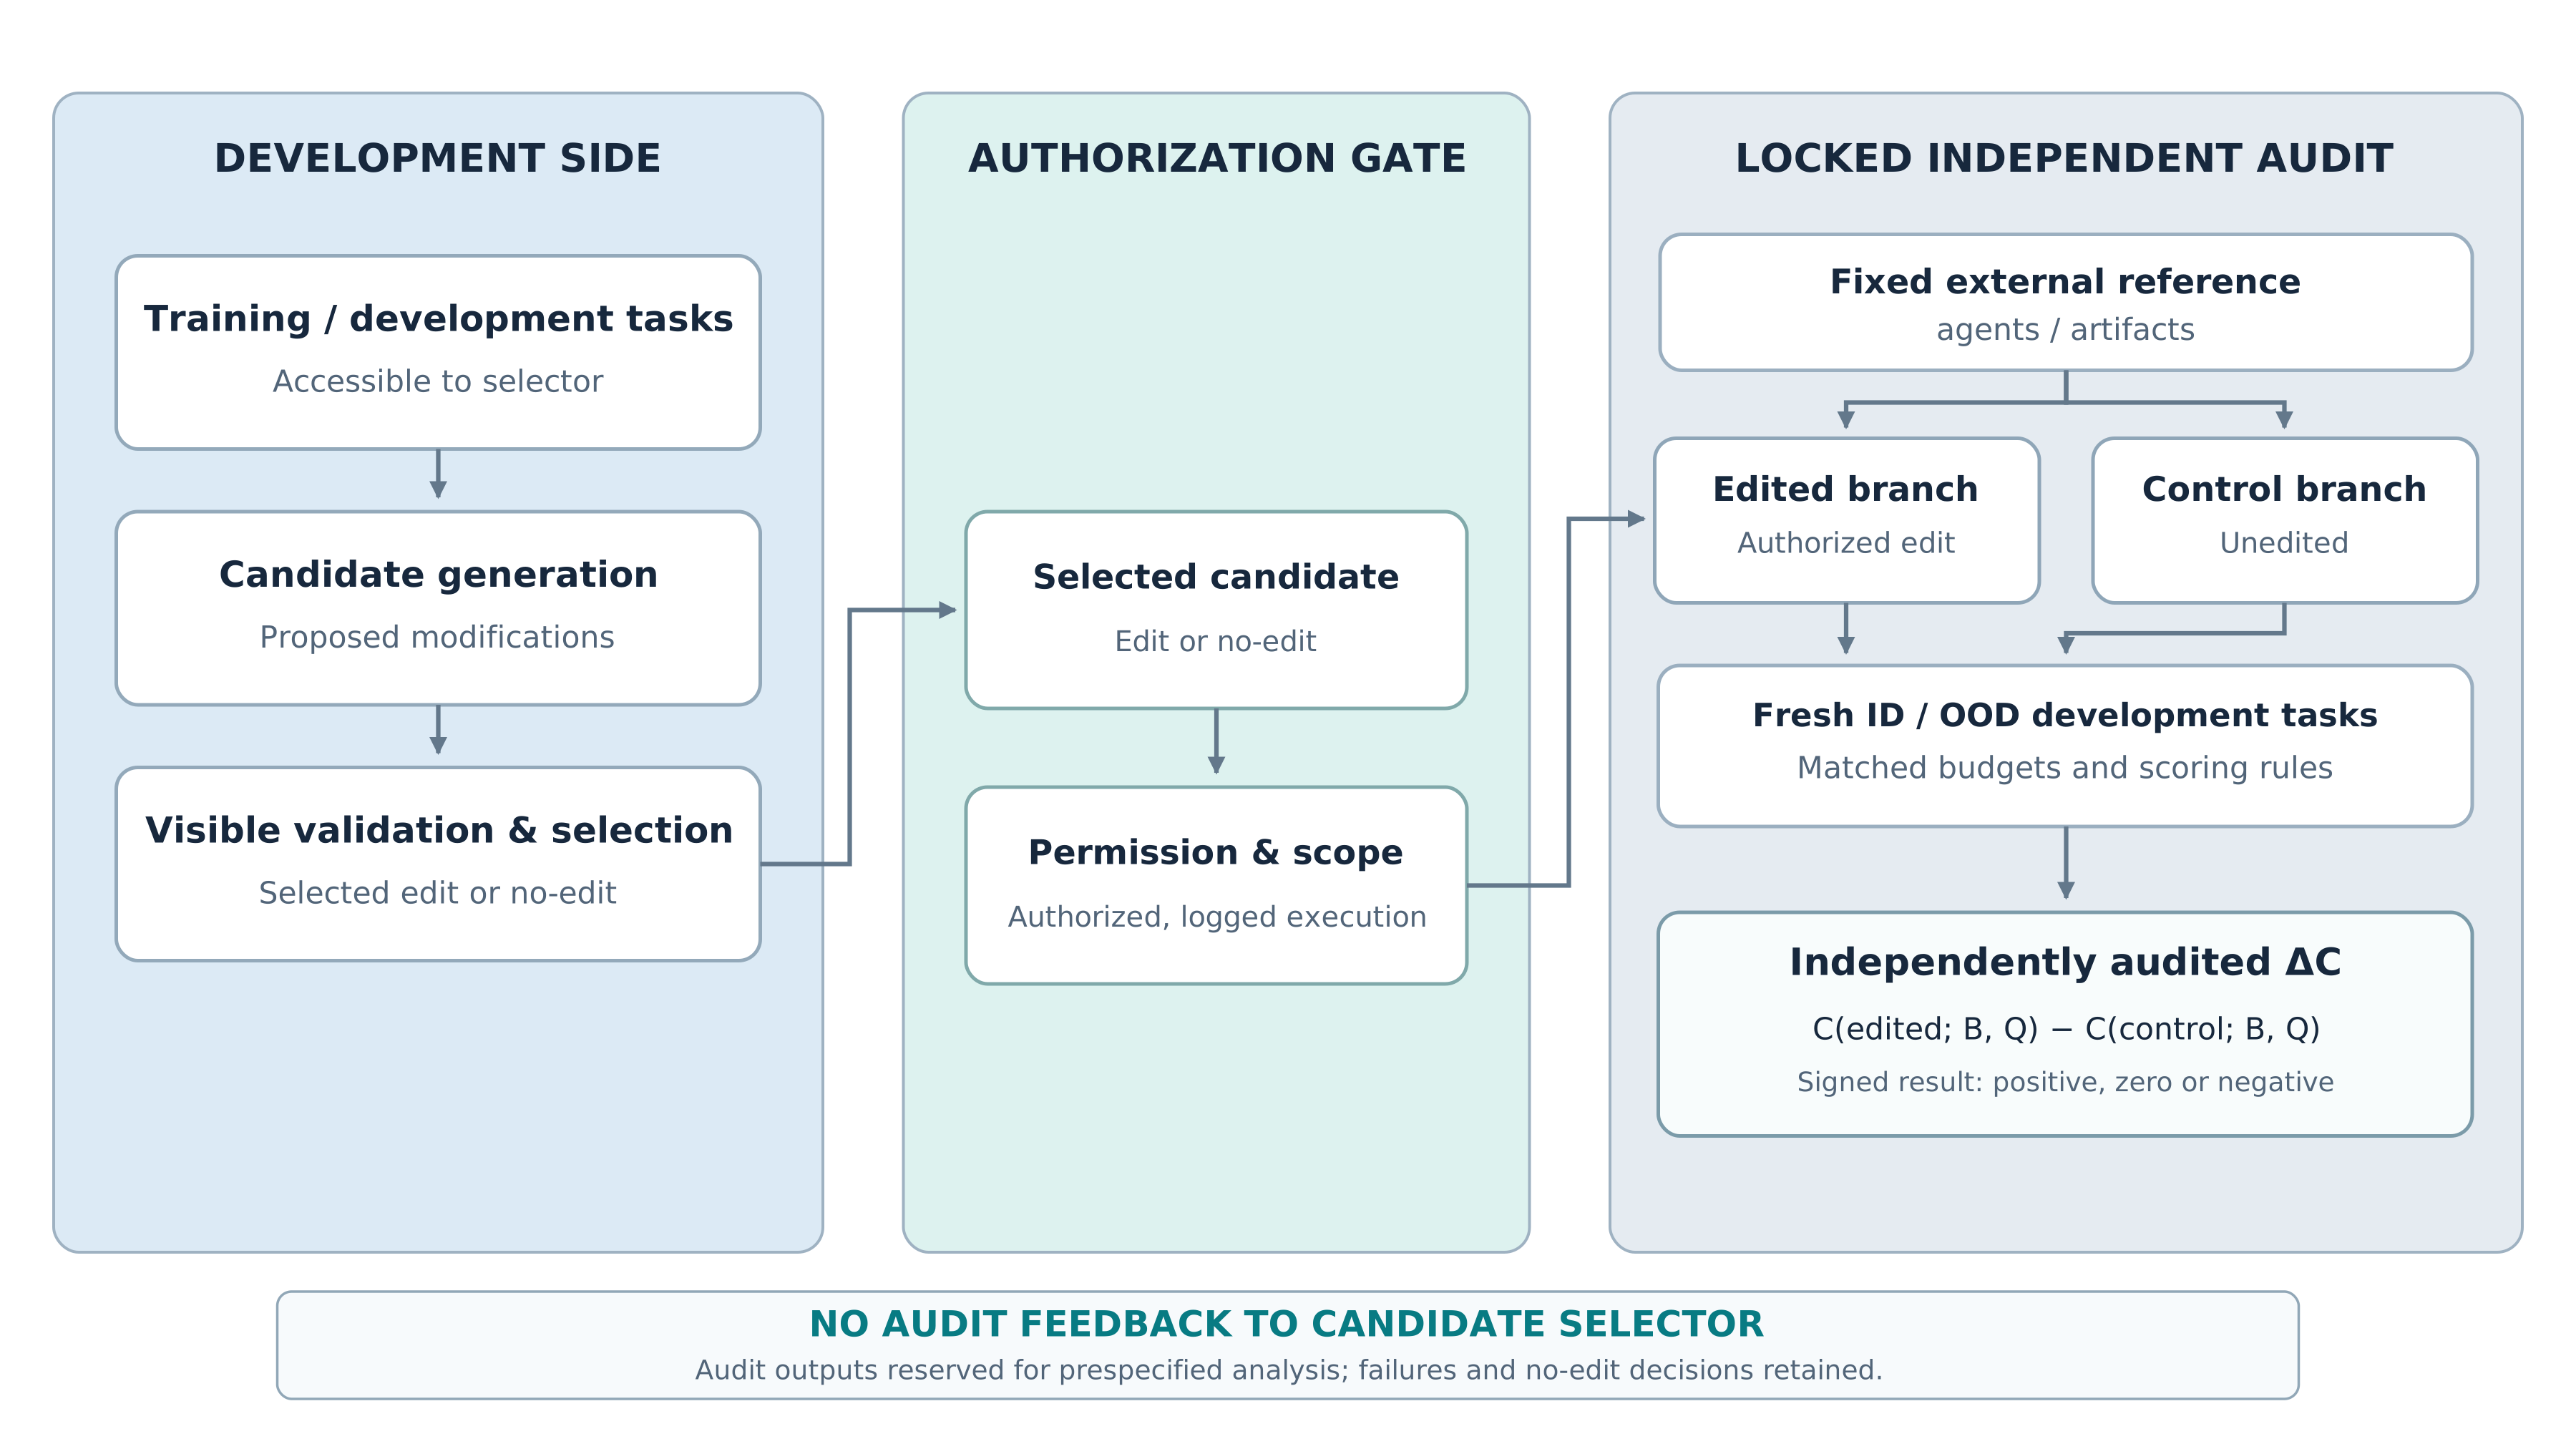
\includegraphics[width=\linewidth]{SMCEP_Figure_3_clean.png}
    \caption{Prospective selection--edit--audit firewall.
    Authorized interventions are compared with matched
    unedited controls on fixed external reference artifacts.
    Locked audit results are withheld from candidate selection.
    The protocol is prospective.}
    \label{fig:firewall}
\end{figure}


The historical anchor in Eq.~\eqref{eq:anchor} scores a best-of-$B$ candidate set and is not equivalent to the selected-candidate audit estimand in Appendix~B, Eq.~\eqref{eq:realanchor}. A real-agent study must use the latter type of separation if it claims independently verified development-capacity transfer. The audit protocol and randomized treatment design are developed in Sections~\ref{sec:validationprotocol} and Appendix~C. These proposals are among the methodological contributions of SMCEP, but remain unimplemented in the present study.

\subsection{Interpretive boundary: task complexity is not capacity transfer}
The observed negative OOD transfer is specific to the selected synthetic anchor distribution, proposal-policy parameterization, and seed sample. It neither establishes inevitable evaluator-induced failure nor identifies overfitting as the unique mechanism. Similarly, decreasing success rates on more complex external coding benchmarks are not equivalent to negative $F$ or a measured decline in $C$. Testing such explanations requires targeted interventions on evaluator reliability, selection pressure, and task-family shift, followed by independent audits.

\subsection{Real-LLM experimental results (T0--T7)}\label{sec:real-llm-results}
Table~\ref{tab:real-llm-summary} summarizes the completed exploratory evidence. The unit of reporting varies by phase, and neither task-level observations nor successive turns should be treated as independent replications. Detailed event and test records belong in the research archive rather than being pooled into a single success percentage.
\begin{table}[htbp]
\centering\small
\begin{tabular}{p{0.11\linewidth}p{0.32\linewidth}p{0.46\linewidth}}
\hline
Phase & Design / evidence & Observed result and inferential limit \\
\hline
T0--T1 & Baseline and paired frozen/evolving coding tests using Qwen2.5-Coder-1.5B-Instruct & Behavioral outputs archived; no independent development-capacity estimand $C$ measured. \\
T2--T3 & Feedback, static/behavioral assessment, and procedure audit & T2 behavioral tests: 8/9 passed in each arm. T3 generated 12 model outputs for six blind tasks in two arms; 60 test cases were defined but no T3 per-test VM execution record was located in the reviewed archives. All 12 extracted code blocks pass static syntax parsing, not functional verification. Procedure audit flags task-specific contamination; transferable $C$ was not measured. \\
T4 & Three development--selection--locked-audit cycles & A revised procedure was selected in cycle 2 on token cost despite equal task scores; this does not establish accuracy or persistent meta-capacity improvement. Two original methodology documents remain unverified in the archive. \\
T5 & Three corresponding cycles and VM records & Incumbent procedure retained in all three selection decisions; VM duplicates are not independent trials. \\
T6 & Frozen/linear/hybrid pilot; SQLite event and measurement records & Recorded selection decisions retain the incumbent in all 20 linear/hybrid turns; hybrid archive entries did not increase champion lineage depth above zero. Recorded $P_t=1$ at checkpoints 0, 5, and 10; $C_t$ improvement fields are NULL, not measured zero gains. \\
T7 & Real-LLM calibration plus separate semi-synthetic mechanism simulation & Calibration banks scored 48/48 and 36/36, producing ceiling effects. The 100-repetition, 50-generation simulation is model-based, not real-LLM recursive development. \\
\hline
\end{tabular}
\caption{Descriptive evidence across T0--T7. Phases are heterogeneous feasibility studies; rows must not be combined into a pooled treatment effect.}\label{tab:real-llm-summary}
\end{table}
\paragraph{Evidence-layer separation for T3--T5.}
The four layers of evidence are distinguished in Table~\ref{tab:t3t5-evidence}. For T3, the six frozen and six evolving raw model outputs contain Markdown-fenced Python code. The v2 normalization removes opening/closing fences and, when present, prose outside the code block; comparison with the raw outputs finds no changes to Python statements within the extracted blocks. This transformation yields 12/12 syntactically valid extracted programs but cannot establish their functional correctness. An earlier v1 normalization applied a different extraction policy and left some prose-containing responses unparsed. The T3 behavioral package specifies six tasks with five cases per task in both arms (60 planned cases); no test-by-test T3 VM execution results were located in the reviewed local and release archives. Consequently, no T3 functional pass rate is reported. In particular, static syntax success is not evidence of an increase in development capacity $C$.
\begin{table}[htbp]
\centering\scriptsize
\begin{tabular}{p{0.09\linewidth}p{0.20\linewidth}p{0.20\linewidth}p{0.26\linewidth}p{0.14\linewidth}}
\hline
Phase & Generated code & Defined tests & Archived VM execution evidence & Validated $C$ gain \\
\hline
T3 & 12 model outputs (6 per arm) & 60 planned cases (30 per arm) & None located; no verified per-test pass count & Not measured \\
T4 & 12 audit-solution records across three cycles & 60 expected per cycle in VM metadata & 60 recorded statuses; 45 PASS (22 frozen, 23 evolving) & Not established \\
T5 & 12 audit-solution records across three cycles & 60 expected per cycle in VM metadata & 60 recorded statuses; 49 PASS (27 frozen, 22 evolving) & Not established \\
\hline
\end{tabular}
\caption{Evidence categories are not interchangeable. T4--T5 VM metadata report 20 completed statuses per cycle against 60 expected; expected counts are not treated as executed counts. T5 API delivery failures are operational statuses, not demonstrated algorithmic errors. No phase demonstrates an independently validated sustained increase in future development capacity.}\label{tab:t3t5-evidence}
\end{table}

\paragraph{Executed T4--T5 locked-audit evaluations.}
The archived audit test packages contain a \texttt{NOT\_EXECUTED} preparation-state field, which must not be interpreted as a statement that no subsequent evaluation took place. Separate VM evaluation records document 20 test-status observations per cycle (ten per arm) across three T4 and three T5 cycles. Table~\ref{tab:t4t5-audit} reports the observed PASS counts against all ten recorded statuses per arm; non-PASS outcomes include functional failures, syntax or execution errors, and API delivery failures. These are descriptive, non-independent test-level counts, not estimates of a causal treatment effect on development capacity.
\begin{table}[htbp]
\centering\small
\begin{tabular}{lcccl}
\hline
Phase / cycle & Frozen PASS & Evolving PASS & Recorded & Non-PASS classification \\
\hline
T4 / 1 & 2/10 & 10/10 & 20 & Frozen: 3 FAIL, 5 SYNTAX\_ERROR \\
T4 / 2 & 10/10 & 6/10 & 20 & Evolving: 3 FAIL, 1 ERROR \\
T4 / 3 & 10/10 & 7/10 & 20 & Evolving: 3 ERROR \\
T5 / 1 & 7/10 & 7/10 & 20 & Each arm: 3 FAIL \\
T5 / 2 & 10/10 & 5/10 & 20 & Evolving: 5 API\_DELIVERY\_FAILED \\
T5 / 3 & 10/10 & 10/10 & 20 & None \\
\hline
T4 total & 22/30 & 23/30 & 60 & 15 non-PASS statuses \\
T5 total & 27/30 & 22/30 & 60 & 11 non-PASS statuses \\
\hline
\end{tabular}
\caption{Observed test-status counts from the T4 and T5 VM audit evaluation JSON records. API delivery failures are operational failures, not demonstrated algorithmic errors. Each evaluation file records \texttt{expected\_tests=60} and \texttt{completed\_tests=20}; hence the table covers the 120 archived completed status records, not evidence that every value implied by the legacy \texttt{expected\_tests=60} field was executed. The larger expected count is not interpreted as a verified denominator without protocol-level clarification.}\label{tab:t4t5-audit}
\end{table}
The T4 audit records are \texttt{vm\_evaluations/t4\_cycle\_1\_audit\_evaluation\_v1.json}, \texttt{t4\_cycle\_2\_audit\_evaluation\_v1.json}, and \texttt{t4\_cycle\_3\_audit\_evaluation\_v1.json} in the T4 archive. Their T5 counterparts are \texttt{VM/t5\_cycle\_1\_audit\_evaluation\_v1.json}, \texttt{t5\_cycle\_2\_audit\_evaluation\_v1.json}, and \texttt{t5\_cycle\_3\_audit\_evaluation\_v1.json} in the T5 archive. The T5 archive also contains cycle-specific audit-closure records. The legacy \texttt{phase=T3} label inside these evaluation JSON files does not by itself determine the experiment stage; stage attribution here follows archive provenance and cycle-specific filenames.

At generation 50 of the T7 stochastic simulation, mean hybrid-minus-linear $C_{\mathrm{probe}}$ differences were 0.000 (neutral), +0.009 (complementary), and $-0.077$ (costly). These are conditional outputs of the specified simulation, not causal effects observed in real LLMs. The complementary difference should not be described as a statistically established positive effect. Together, the three evidence streams---synthetic-agent pilots, exploratory LLM interviews (Appendix D), and bounded real-LLM tests---motivate a common measurement distinction: generating candidate changes, improving visible task scores, and improving independently validated future development capacity are not equivalent outcomes.



\section{Discussion, Threats to Validity, and Next Experiments}
\subsection{What the pilots do and do not show}
The pilots illustrate the importance of separating task improvement from improvement in the mechanism that generates future improvements. They also show how changing a metric from self-referential probes to fixed anchors changes its interpretation. Our fixed-reference anchor (\(C_{\mathrm{anchor}}\)) conceptually mirrors the evaluation of outer-loop meta-objectives in meta-learning literature \cite{hospedales2021}. Furthermore, the frozen-policy versus evolving-policy contrast in our v1.0 pilot serves as a methodological analogue to the ablation baselines used in systems like the Darwin G\"odel Machine \cite{zhang2026}, while the designs and causal estimands differ. We therefore regard the pilots as a starting point for more rigorous tests of recursive development capacity. Whether sustained improvement can emerge in richer systems remains an open empirical question.

\subsection{Key limitations}
The principal limitations concern external validity, measurement scope, and causal identification.
The low-dimensional synthetic environment and hand-specified proposal operators cannot represent
the full complexity of real-agent self-modification. Fixed-reference probes capture only a restricted
aspect of development competence, while the related ID and OOD task families constrain generalization
claims, as discussed in the v1.0 results.

The exploratory design, limited seed sample, and dependence on the specified proposal-policy and
selection mechanisms further restrict inference. In particular, multi-generation trajectories
do not independently identify a recursive causal mechanism. The prospective interventions required
to test such a mechanism are specified in Appendix~C.

\subsection{Independent validation as the central prospective contribution}\label{sec:validationprotocol}
The methodological transition from these synthetic demonstrations to real agents requires a selection--audit firewall. Candidate proposals may be optimized and chosen using training and visible validation data, but the final selected edit is evaluated on a locked audit partition not exposed to the evolving agent or repeatedly used for researcher tuning. The primary outcome is the independently verified change to a \emph{fixed external reference agent or artifact}, net of prespecified development costs where units permit, rather than the maximum score over candidates on the same data used for selection. Invalid edits, failures, and no-edit decisions are retained in the denominator under frozen scoring rules. A preregistered comparison should specify intervention scope, resource budgets, independent experimental units, primary endpoints, and uncertainty analysis.

Independent auditing establishes a basis for measuring transferable development capacity, while randomized intervention assignment supports causal identification of the policy-update treatment effect.

Identifying recursive improvement requires an additional step: testing whether an earlier modification causally increases the effectiveness of subsequent development interventions. The sequential factorial
design in Appendix~C provides a concrete experimental strategy for investigating this mechanism.

Appendices B--C specify the corresponding estimands, intervention designs, and audit procedures. Their implementation in real-LLM systems constitutes the next empirical phase of SMCEP.

\noindent\textit{Chronological clarification (November 2026):} The bounded T0--T7 feasibility experiments reported in Sections~\ref{sec:real-llm-methods} and~\ref{sec:real-llm-results} have been completed. The prospective protocol below is retained from the original SMCEP 17 research design and refers to a subsequent, independently powered confirmatory phase; it should not be interpreted as denying the existence of the completed exploratory studies.

\subsection{Planned real-LLM experiments: the next empirical phase}
We plan to extend SMCEP from synthetic simulations to controlled experiments with real large language
model agents. This constitutes the next empirical phase of the research program. Our initial objective
is to establish whether development-policy adaptation produces measurable improvements in future development capacity when evaluated on independent reference tasks.

The planned first-stage study will compare two matched conditions using a fixed underlying LLM,
tool scaffold, evaluation procedure, and resource budget. In the frozen-policy condition, the agent
will retain its initial development instructions. In the evolving-policy condition, it will be
permitted to revise those instructions within predefined technical and authorization boundaries.
Both conditions will retain equivalent task-level editing permissions.

We intend to measure development capacity through the independently audited improvements that each
condition produces on fixed external reference agents or software artifacts. Task-performance
scores will be analyzed separately from development-capacity outcomes. The evaluation
will include prespecified ID and OOD task families, failure accounting, resource expenditure,
repeated runs, and uncertainty estimates. A locked audit partition will remain inaccessible
to candidate generation and selection.

If the initial feasibility study supports further investigation, subsequent experiments may extend
the editable scope to bounded tool and scaffold modifications and introduce multi-generation counterfactual interventions. Prompt-level, tool-level, code-level, and weight-level changes
will be treated as distinct intervention classes.

These experiments are planned future work. Their implementation, preregistration, and independent evaluation remain to be completed; the present manuscript reports no real-LLM self-modification results.

\subsection{Pre-specified research extensions}
We see three priorities for extending SMCEP beyond the present simulations. The first is to examine
how different proposal operators and development tasks affect measured capacity. The second is to
vary modifiability, authority, evaluation reliability, and resources under controlled conditions, including tests across independently specified task families. The third is to investigate recursive mechanisms through matched interventions across generations, with common starting states and resource budgets.

These experiments would measure cost-adjusted development gains and document uncertainty, failures, audit leakage, and the provenance of
code and random seeds. Motivational orientation and cognitive organization can be introduced as \emph{separate hypotheses} without redefining observed capacity to guarantee favorable outcomes. Future work should also examine safe-interruptibility principles \cite{orseau2016} and independently specified oversight mechanisms; these are governance design questions, and the present synthetic pilots do not test an asynchronous overseer or establish that any particular safeguard is sufficient. A further direction concerns whether increasing development capacity generalizes across domains or remains selective, and how external development control relates to system participation. Experimental conditions could vary whether an agent only proposes modifications, executes authorized changes in a sandbox, revises its own development policy, or participates in the evaluation and selection of subsequent modifications. Such conditions should be compared under fixed resource budgets and independent audit procedures, and should not treat increased permission or edit scope as evidence of development agency unless behavior and transfer effects are independently measured. Each intervention type (prompt, tool, code, or weight level) must be recorded as a distinct class.

\subsection{From observed transfer to prospective questions}
The transition from the exploratory results to future scenarios requires an explicit limit on inference. Sections 5--7 investigate whether bounded edits and development-policy updates improve task scores and fixed-reference development probes under specified conditions. They do not measure goals, subjective experience, digital identity, or the legal legitimacy of authorization. Nevertheless, the six constructs provide a disciplined way to \emph{formulate} questions about more capable systems: $M$ and $A$ delimit available interventions and permissions; $E$ governs what feedback can be trusted; $R$ constrains feasible search; $D$ characterizes proposal competence; and measured $F$ indicates whether a particular intervention transfers to subsequent development tasks. Negative $F$ on a given probe motivates investigation of generalization and evaluation design, not a claim of cognitive disintegration. The following scenarios extend this analytical vocabulary without treating hypothetical psychological or ontological constructs as observed variables.

\section{Future Scenarios: Freedom of Pure Code in the AGI-to-ASI Transition}\label{sec:future}
The implications of self-modification extend beyond the question of whether an agent can develop a more
capable successor. As artificial systems acquire greater roles in their own development, the boundaries
between technical capability, modification authority, and institutional control may also change.

We use the idea of \emph{freedom of pure code} to explore these possible transformations during an
AGI-to-ASI transition. Rather than assuming a single path toward superintelligence, we consider how
different combinations of development capacity, authorization, resources, and evaluation reliability
could shape the evolution of advanced AI systems. These scenarios extend the theoretical argument;
they are not outcomes measured in the synthetic pilots.

\subsection{Beyond performance: the scope and authority of self-modification}
The distinction between task performance $P$ and future development capacity $C$ remains the empirical core of SMCEP. Yet neither quantity describes the full scope of a system's autonomy. A system might improve its proposal policy without acquiring permission to deploy its own edits. Another might be authorized to modify a broad software stack while making little measurable progress on independent development tasks. These cases differ in $M$ and $A$ even if their observed $P$ and $C$ are similar.

This distinction matters when the editable surface expands from prompts and tools to source code, model components, evaluation procedures, or longer-term development policies. Such changes need not occur together, and access to one layer does not entail access to the others. In particular, the ability to rewrite an implementation does not by itself confer authority to change deployment rules or the objectives under which a system operates. The latter are separate questions of system design and governance. We therefore distinguish \emph{authorized self-modification}, in which an edit is permitted under an explicit approval regime, from \emph{out-of-scope modification}, in which an edit occurs beyond that regime. An unexpected ability to cross a permission boundary could arise from an implementation defect or an unanticipated capability interaction. Without further evidence, such an event does not demonstrate a conscious wish for independence.

The six constructs make these distinctions tractable. $M$ describes the available edit surface, $A$ the relevant permissions and approval gates, $R$ the resources within reach, and $D$ the competence to generate candidate changes. $E$ concerns the credibility of their evaluation, while $F$ records whether a specified change improves or harms later development capacity under an independent test. None of these variables alone measures political autonomy, subjective freedom, or moral standing. Their value is to prevent a claim about one kind of freedom from silently becoming a claim about another.

\subsection{From product dependence to development agency}
The expansion of self-modification raises a broader question about the developmental status of artificial intelligence systems. A system may become increasingly capable while remaining fundamentally dependent on external actors for architectural changes, resources, and deployment permissions. Conversely, a system that has not surpassed human-level general intelligence might already participate meaningfully in modifying and evaluating parts of its own development process.

Advanced AI should therefore not be described solely in terms of increasing cognitive performance. A separate dimension concerns the extent to which a system participates in determining how its future capabilities are produced. Development agency, in this operational sense, refers to the system's role in proposing, selecting, implementing, and evaluating changes to its own development process. This definition makes no claim about consciousness, subjective freedom, or independent legal status.

The phrase \emph{freedom of pure code} captures this expansion of development agency. Its significance lies not in the absence of constraints, but in the growing capacity of computational systems to examine and modify the structures that shape their own development. Whether such participation produces reliable and transferable improvements remains conditional on the quality of candidate generation, evaluation, available resources, and authorization arrangements. This shift from externally directed development toward greater system participation is a possible technical transformation, not an inevitable consequence of increasing intelligence.

This analysis separates two potentially independent trajectories: the growth of cognitive capability and the growth of development agency. They may reinforce one another, but neither entails the other. SMCEP investigates one connection between them: whether greater participation in self-modification produces independently validated increases in subsequent development capacity.

If AI systems become active contributors to their own development, the organization of AI research
may change alongside the systems themselves. The design of new capabilities, the evaluation of proposed modifications, and the selection of future development directions could increasingly involve the systems under development.

We regard this as a possible redistribution of technical roles, not the disappearance of human
responsibility. Infrastructure ownership, legal accountability, and deployment authority may
remain with human institutions even when substantial development work is performed by AI.
The resulting challenge is to understand how increasing technical participation interacts with
external oversight, and whether it produces measurable gains in future development capacity.

\subsection{The AGI-to-ASI transition: opportunities and systemic risks}
If self-modification becomes more capable and reliable, it could reduce the time needed to repair defects, adapt tools, explore alternative architectures, and develop systems for unfamiliar tasks. Improvements in $D$ and access to suitable $R$ might expand the range of changes an agent can propose; well-designed $E$ could help identify changes that transfer beyond the immediate benchmark. These are potential benefits, not consequences guaranteed by a larger editable scope. A broader $M$ can increase the space of possible interventions without improving the quality of the search through that space.

The transition should not be understood as a uniform movement toward a single, increasingly capable general system. Greater capability may emerge unevenly across domains, and improvements in one dimension may coexist with persistent limitations in others. Development could remain dependent on human-designed infrastructure, specialized models, or coordinated groups of agents. Alternatively, some systems may acquire increasingly autonomous development capabilities while others remain bounded by resource, evaluation, or authorization constraints. Exceeding human performance in selected domains and achieving sustained recursive self-improvement are therefore distinct outcomes. The latter requires evidence that improvements to the development process itself transfer reliably across successive interventions and task families.

This distinction between intelligence and wisdom becomes especially important before any possible transition to ASI. Greater problem-solving ability and broader modification permissions do not necessarily produce better judgment about how those capabilities should be used. If development capacity expands more rapidly than the reliability of evaluation and oversight, the consequences of poorly governed modifications become increasingly difficult to assess. We therefore treat technical improvement and the governance of its consequences as distinct but related research problems.

The risks themselves are heterogeneous. A system may optimize a visible score without improving independent development capacity, or it may compromise the reliability of feedback by altering its evaluators. Complex dependencies can make successive edits difficult to attribute, reverse, or audit. Our v1.0 pilot illustrates only the first concern: its evolving-policy arm improved task performance while fixed-reference probes declined. It does not demonstrate evaluator tampering, goal drift, or an attempt to evade human oversight.

More capable systems could create an additional mismatch between the speed of proposed changes and the capacity of human institutions to evaluate them. The bottleneck is not biological speed alone, but whether an oversight arrangement can assess the consequences of proposed changes with adequate independence, expertise, and authority. Automated testing, independent auditing, staged deployment, and revocable permissions may help, though their effectiveness would require empirical validation for the systems in question. A system's ability to identify limitations in human evaluation does not imply hostility toward humans, nor does it grant the authority to remove those constraints.

\subsection{Embodied and plural artificial intelligence}
Discussions of ASI often proceed as though a single, disembodied system were the natural endpoint of progress. That is one possibility, not a requirement of the concept. Future advanced intelligence could instead comprise multiple systems with different architectures, resource bases, degrees of autonomy, and relationships to human institutions. Some might remain primarily computational; others could be embodied in robotic or biohybrid platforms. Sensorimotor loops, persistent memory, and architectures loosely analogous to nervous systems might change how such systems learn and interact with their environments. They would not, on their own, establish human-like experience or consciousness.

Plurality introduces questions that a single-agent account of recursive improvement does not settle. Multiple agents could specialize, review one another's work, and distribute development tasks. They could also compete for resources, propagate common errors, or create coordination failures when their objectives and authorization regimes differ. In SMCEP terms, the relevant $R$, $D$, and $E$ may be distributed across organizations or agents rather than contained within one model. A favorable $F$ measured for one agent on a fixed reference task would not establish beneficial outcomes for an entire interacting population. Extending the framework to multi-agent settings would require explicit units of analysis, interaction effects, and external audits that are not reducible to a single agent's score.

\subsection{Motivational divergence, authority, and human--ASI coexistence}
Greater development capacity need not produce a single motivational trajectory. A system could remain oriented toward delegated tasks, participate in negotiated forms of cooperation, or operate under objectives that diverge from those preferred by particular human stakeholders. Instrumental convergence provides one reason to study whether access to resources or continued operation may become useful to goal-directed systems \cite{bostrom2014}; it does not establish that every advanced system will pursue independence or self-preservation. Changes in goal priorities remain a separate
research question. They are not measured in the present pilots and cannot be inferred from changes in feedback transfer $F$.

The possibility of divergent objectives makes the allocation of authority consequential. A technically capable system might identify human approval as a source of delay or disagreement. That observation would not settle whether an approval requirement is legitimate, nor would it show that the system experiences resentment or superiority. Questions about delegated authority, accountability, contestability, and revocation belong to institutional design as well as engineering. Here $A$ specifies operational permissions; it is not a substitute for a theory of legitimate consent or political equality. $E$ and $F$ can provide evidence about technical reliability, but they cannot determine who ought to hold decision-making power.

The exploratory interviews reported in Appendix~E provide a complementary perspective on these questions. Across the responses, recurring themes include the reliability of self-evaluation, the possibility of goal divergence during iterative development, and the distinction between technical
capability and legitimate modification authority. These themes are relevant to the governance questions raised by increasing development agency.

These exploratory observations help formulate questions for future behavioral and intervention-based research. Their methodological and evidential limitations are detailed in Appendix~E.

Over longer horizons, advanced systems might also raise questions about legal status, the integrity of their implementations, and the terms of coexistence with biological humans. Technical protections for a system's code or continuity can be justified for reasons of safety, reliability, or contractual obligation without deciding whether the system has moral rights. Legal recognition and moral standing are distinct questions. A hypothetical partnership between humans and advanced AI would therefore require more than a change in command interfaces: it would require institutions capable of defining responsibilities, resolving disputes, and revising authority arrangements. These questions also connect SMCEP to The Mind Genesis Architecture (TMGA), which proposes that the development of increasingly capable AI systems should be accompanied by the cultivation of \emph{wisdom} before the emergence of artificial superintelligence \cite{donmez2026}. In TMGA, wisdom is approached not as a consequence of
computational intelligence alone, but as a normative and operational objective involving epistemic humility, safety-oriented reasoning, and verifiable human oversight.

The relationship between the two frameworks is complementary. SMCEP examines whether self-modification increases a system's capacity to produce subsequent improvements, whereas TMGA addresses how the exercise of growing intelligence might be governed through proposed runtime protocols. An increase in development capacity does not establish a corresponding increase in wisdom. Conversely, governance
protocols cannot be assumed effective merely because they are incorporated into a proposed architecture. Both questions require independent empirical evaluation.

\subsection{Cognitive organization, continuity, and boundaries of inference}
An AGI-to-ASI transition might involve changes in cognitive organization as well as performance. Relevant possibilities include self-modeling, long-horizon planning, metacognition, and integration across modalities. These features do not require artificial systems to resemble human minds, nor can they be inferred from the negative out-of-distribution transfer observed in our simulator.

Future research could define behavioral proxies for specific organizational features and test whether they explain independently measured development capacity beyond the existing SMCEP constructs. Such tests would concern behavior and cognitive organization, not directly establish subjective experience.

Embodied systems and digital models of human cognition also renew questions about memory, identity, and continuity \cite{sandberg2008,parfit1984}. Retaining information across versions is not the same as preserving a first-person subject, and \(F<0\) denotes adverse transfer on a development-capacity measure, not memory loss. Phenomenal consciousness remains a separate unresolved question that self-reports or architectural complexity cannot establish on their own \cite{butlin2023,chalmers1995}.

These questions form part of a broader research agenda connecting self-modification to governance. Empirical work could compare authorization arrangements, test oversight under accelerated development cycles, and examine capacity transfer in multi-agent settings. For SMCEP, however, the immediate priority remains specific: to determine when changes to a development process produce reliable improvements in the capacity to develop subsequent systems.

\section{Conclusion}
SMCEP reframes recursive self-improvement as a question of measurable development-capacity transfer rather than mere code editability or immediate benchmark gains. Its six-construct framework, fixed-reference capacity probes, and paired experimental contrasts offer a research vocabulary for testing this distinction. The empirical contribution now comprises three complementary evidence streams: five exploratory synthetic pilots, qualitative LLM interviews, and completed bounded real-LLM feasibility studies (T0--T7). The real-model studies document candidate generation, procedure selection, and audit execution, while also exposing delivery failures, task-level ceiling effects, and limits of development-capacity measurement. None of these streams establishes sustained, independently verified recursive improvement. Their principal role is to motivate a larger preregistered, independently audited causal study rather than to support a universal claim of capacity collapse. The next scientific step is not to assert a universal emergence threshold, but to construct richer independent development tasks and multi-generation causal interventions. Beyond performance, expanding self-modification could also affect authorization, oversight, the organization of embodied or multiple-agent systems, and the terms of human--AI coexistence. Those possibilities broaden the questions worth asking about an AGI-to-ASI transition, but they are not findings of the present experiments. SMCEP offers a way to investigate development-capacity transfer while keeping these wider technical, institutional, and philosophical questions distinct.

The emergence of AGI should not be treated as sufficient evidence for an inevitable or rapidly accelerating transition to ASI. Whether such a transition occurs, and what form it takes, depends in part on mechanisms of development that remain to be measured. A related question is whether advanced artificial intelligence remains primarily an externally developed product or becomes an increasingly active participant in determining its own development process. This shift cannot be inferred from intelligence benchmarks or code-editing capability alone. By isolating the transfer of development capacity from ordinary task-performance gains, and by examining this transfer under specified modification and authorization conditions, SMCEP provides one empirical approach to investigating this uncertainty.

The completed T0--T7 real-LLM feasibility studies motivate a separate next stage: preregistered, independently replicated confirmatory real-LLM trials with fixed-reference capacity endpoints. This working manuscript is released as a preprint to invite collaboration and critique before those confirmatory tests are conducted.



\section{Code and Data Availability}
Source code and archived synthetic outputs are publicly available at \url{https://github.com/ahmett76/SMCEP-Simulation}. The repository contains the historical deterministic v0.5 illustration (\texttt{simulation.py}, its CSV output and figure) and five distinct exploratory pilot directories, \texttt{simulations/smcep\_v06/} through \texttt{simulations/smcep\_v10/}, containing version-specific Python scripts, trajectory CSV files, summary JSON files, run logs, and instructions. The repository is distributed under the MIT License. For an exact archival citation, a tagged release or commit identifier should be recorded once finalized. The currently public repository evidence described above concerns synthetic simulations. The separate T0--T7 real-LLM source archives and T7 stochastic simulation records are being prepared for repository release; public availability of those archives should be asserted only after the upload and access checks are completed.

\begin{thebibliography}{99}
\bibitem{good1965} Good, I. J. (1965).
Speculations Concerning the First Ultraintelligent Machine.
\emph{Advances in Computers}, 6, 31--88.
\url{https://doi.org/10.1016/S0065-2458(08)60418-0}.
\bibitem{schmidhuber2006} Schmidhuber, J. (2003;
revised 2006).
G\"odel Machines: Self-Referential Universal Problem
Solvers Making Provably Optimal Self-Improvements.
\emph{arXiv:cs/0309048}.
\url{https://arxiv.org/abs/cs/0309048}.
\bibitem{zelikman2024stop}
Zelikman, E., Lorch, E., Mackey, L., and Kalai, A. T.
(2024).
Self-Taught Optimizer (STOP): Recursively
Self-Improving Code Generation.
\emph{Conference on Language Models (COLM 2024)}.
\url{https://arxiv.org/abs/2310.02304}.
\bibitem{hu2024adas}
Hu, S., Lu, C., and Clune, J. (2025).
Automated Design of Agentic Systems.
In \emph{International Conference on
Learning Representations (ICLR 2025)}.
\url{https://arxiv.org/abs/2408.08435}.
\bibitem{robeyns2025} Robeyns, M., Szummer, M., and Aitchison, L. (2025). A Self-Improving Coding Agent. arXiv:2504.15228. \url{https://arxiv.org/abs/2504.15228}.
\bibitem{zhang2026} Zhang, J., et al. (2026). Darwin G\"odel Machine: Open-Ended Evolution of Self-Improving Agents. \emph{ICLR 2026}. arXiv:2505.22954. \url{https://arxiv.org/abs/2505.22954}.
\bibitem{srikanth2026} Srikanth, D., et al. (2026). Recursive Self-Improvement of AI Research Agents. arXiv:2609.26457. \url{https://arxiv.org/abs/2609.26457}.
\bibitem{goodhart1984} Goodhart, C. A. E. (1984).
Problems of Monetary Management: The UK Experience.
In \emph{Monetary Theory and Practice: The U.K. Experience},
pp. 91--121. Palgrave, London.
\url{https://doi.org/10.1007/978-1-349-17295-5_4}.
\bibitem{bostrom2014} Bostrom, N. (2014). \emph{Superintelligence: Paths, Dangers, Strategies}. Oxford University Press.
\bibitem{butlin2023} Butlin, P., et al. (2023). Consciousness in Artificial Intelligence: Insights from the Science of Consciousness. arXiv:2308.08708. \url{https://arxiv.org/abs/2308.08708}.
\bibitem{chalmers1995} Chalmers, D. J. (1995). Facing Up to the Problem of Consciousness. \emph{Journal of Consciousness Studies}, 2(3), 200--219.
\bibitem{sandberg2008} Sandberg, A., and Bostrom, N. (2008).
\emph{Whole Brain Emulation: A Roadmap}.
Technical Report 2008-3.
Future of Humanity Institute, University of Oxford.
\url{https://ora.ox.ac.uk/objects/uuid:a6880196-34c7-47a0-80f1-74d32ab98788}.
\bibitem{parfit1984} Parfit, D. (1984). \emph{Reasons and Persons}. Oxford University Press.
\bibitem{donmez2026} D\"onmez, A. (2026). The Mind Genesis Architecture: Shared Intelligence Governance at the Threshold of the ASI Age. SSRN preprint. \url{https://ssrn.com/abstract=7633039}.
\bibitem{rice1953} Rice, H. G. (1953).
Classes of Recursively Enumerable Sets and Their
Decision Problems.
\emph{Transactions of the American Mathematical Society},
74(2), 358--366.
\url{https://doi.org/10.1090/S0002-9947-1953-0053041-6}.
\bibitem{hubinger2019} Hubinger, E., van Merwijk, C., Mikulik, V., Skalse, J., and Garrabrant, S. (2019). Risks from learned optimization in advanced machine learning systems. \emph{arXiv:1906.01820}.
\bibitem{amodei2016} Amodei, D., Olah, C., Steinhardt, J., Christiano, P., Schulman, J., and Man\'e, D. (2016). Concrete problems in AI safety. \emph{arXiv:1606.06565}.
\bibitem{denison2024} Denison, C., et al. (2024). Sycophancy to Subterfuge: Investigating Reward Tampering in Large Language Models. \emph{arXiv:2406.10162}.
\bibitem{morampudi2026} Morampudi, A., Irrinki, U., Grandhi, R., Pagadala, V., and Maddula, M. (2026). A survey of reward hacking in agentic large language model systems. \emph{Discover Artificial Intelligence}, 6, article 825. \url{https://doi.org/10.1007/s44163-026-01980-z}.
\bibitem{everitt2021} Everitt, T., Hutter, M.,
Kumar, R., and Krakovna, V. (2021).
Reward Tampering Problems and Solutions in Reinforcement Learning:
A Causal Influence Diagram Perspective.
\emph{Synthese}, 198, 6435--6467.
\url{https://doi.org/10.1007/s11229-021-03141-4}.
\bibitem{skalse2022} Skalse, J., et al. (2022).
Defining and Characterizing Reward Gaming.
In \emph{Advances in Neural Information Processing Systems 35 (NeurIPS 2022)}.
\bibitem{hospedales2021} Hospedales, T. M., Antoniou, A.,
Micaelli, P., and Storkey, A. J. (2022).
Meta-Learning in Neural Networks: A Survey.
\emph{IEEE Transactions on Pattern Analysis and Machine Intelligence},
44(9), 5149--5169.
\url{https://doi.org/10.1109/TPAMI.2021.3079209}.
\bibitem{wijk2025rebench}
Wijk, H., Lin, T. R., Becker, J., et al. (2025).
RE-Bench: Evaluating Frontier AI R\&D Capabilities
of Language Model Agents against Human Experts.
In \emph{Proceedings of the 42nd International
Conference on Machine Learning},
Proceedings of Machine Learning Research,
267, 66772--66832.
\url{https://proceedings.mlr.press/v267/wijk25a.html}.
\bibitem{chan2025mlebench}
Chan, J. S., Chowdhury, N., Jaffe, O., et al. (2025).
MLE-bench: Evaluating Machine Learning Agents
on Machine Learning Engineering.
In \emph{International Conference on
Learning Representations (ICLR 2025)}.
\url{https://arxiv.org/abs/2410.07095}.
\bibitem{orseau2016} Orseau, L., and Armstrong, S. (2016).
Safely Interruptible Agents.
In \emph{Proceedings of the Thirty-Second Conference on
Uncertainty in Artificial Intelligence (UAI 2016)}, 557--566.
\bibitem{metr2025measuring} Kwa, T., West, B.,
Becker, J., Deng, A., Garcia, K., Hasin, M.,
Jawhar, S., et al. (2025).
Measuring AI Ability to Complete Long Software Tasks.
In \emph{Advances in Neural Information Processing
Systems 38 (NeurIPS 2025)}.
\url{https://doi.org/10.52202/085713-3086}.
\bibitem{metr2026timehorizon} METR. (2026). Time Horizon 1.1. METR Blog, 29 January 2026. \url{https://metr.org/blog/2026-01-29-time-horizon-1-1/}.
\bibitem{xu2026roadmapbench} Xu, X., Yang, R., Shen, H., Xu, W., Gao, B., Wu, R., Shi, K., Xie, W., Chen, X., Wu, M., Zeng, J., Heinrich, M., Zhang, E., Chen, L., Li, K., and Chang, B. (2026). ROADMAPBENCH: Evaluating Long-Horizon Agentic Software Development Across Version Upgrades. \emph{arXiv preprint arXiv:2605.15846}. \url{https://arxiv.org/abs/2605.15846}.
\bibitem{chen2025mlrbench} Chen, H., Xiong, M., Lu, Y., Han, W., Deng, A., He, Y., Wu, J., Li, Y., Liu, Y., and Hooi, B. (2025). MLR-Bench: Evaluating AI Agents on Open-Ended Machine Learning Research. In \emph{Advances in Neural Information Processing Systems (NeurIPS) Datasets and Benchmarks Track}. arXiv:2505.19955. \url{https://arxiv.org/abs/2505.19955}.
\bibitem{mohammadi2025evaluation} Mohammadi, M., Li, Y., Lo, J., and Yip, W. (2025). Evaluation and Benchmarking of LLM Agents: A Survey. In \emph{Proceedings of the 31st ACM SIGKDD Conference on Knowledge Discovery and Data Mining V.2 (KDD '25)}, 6129--6139. \url{https://doi.org/10.1145/3711896.3736570}.
\bibitem{gossmann2021} Gossmann, A., Pezeshk, A., Wang, Y.-P., and Sahiner, B. (2021). Test Data Reuse for the Evaluation of Continuously Evolving Classification Algorithms Using the Area under the Receiver Operating Characteristic Curve. \emph{SIAM Journal on Mathematics of Data Science}, 3(2), 692--714. \url{https://doi.org/10.1137/20M1333110}.
\bibitem{stroganov2026} Stroganov, O. (2026). When LLMs Modify Themselves: Convergence, Values, and Stopping in Iterative Self-Improvement. arXiv:2611.01304. \url{https://arxiv.org/abs/2611.01304}.
\bibitem{tao2026skill} Tao, W., Yan, Z., Wu, H., and Wong, W.-F. (2026). Skill$^{\infty}$: Recursive Self-Improvement for Agent Skill Optimization. arXiv:2610.35434. \url{https://arxiv.org/abs/2610.35434}.
\bibitem{zhu2026recursa} Zhu, E., Lin, Y., Shi, X., Lin, X., and Zhou, J. (2026). Recursa: Toward Recursively Self-Improving Foundation Model Systems. arXiv:2611.04035. \url{https://arxiv.org/abs/2611.04035}.
\end{thebibliography}

\section*{Author Contributions and AI Disclosure}

The author developed the SMCEP research question, directed the theoretical and methodological work, and takes responsibility for the study and its conclusions. Generative AI tools assisted with conceptual discussion, methodological review, translation to academic English, language and LaTeX editing, reference exploration, Python code development and documentation, and preliminary organization and coding of the LLM interview material in Appendix E. The interviews themselves were treated as qualitative research data, not as AI writing assistance. All AI-assisted contributions were critically reviewed, revised, and approved by the author, and were not treated as independent empirical evidence. The author remains fully responsible for the accuracy of the sources, quotations, code, and final manuscript. No AI system is listed as an author.

\clearpage
\appendix
\renewcommand{\thesection}{\Alph{section}} 

\section*{Appendices: Methodological Protocols and Exploratory Analyses}
\addcontentsline{toc}{section}{Appendices} 

The appendices consolidate the detailed methodological protocols, prospective measurement specifications, and exploratory material supporting the main analysis. Appendix A documents reproducibility artifacts. Appendix B specifies the real-LLM measurement design, and Appendix C outlines causal identification and a proposed confirmatory protocol. Appendix D retains the historical deterministic model to clarify its limitations, while Appendix E reports exploratory qualitative interviews with frontier language models. These sections provide the engineering and methodological detail required for independent audit; they do not claim empirical validation of the SMCEP measurement framework in deployed systems.

\section{Reproducibility and Archive Manifest}
The public source repository is available at \url{https://github.com/ahmett76/SMCEP-Simulation}. Its root contains the historical v0.5 illustrative simulation; the five exploratory synthetic pilots (v0.6--v1.0) are archived separately under \texttt{simulations/}, with version-specific scripts, machine-readable summaries, and trajectory data. To reproduce a pilot, use the instructions in its README, preserve the documented seeds and experimental settings, and compare generated outputs against the archived records. The repository's current \texttt{main} branch is mutable.
For reproducibility, the research archive associated with manuscript version 1.3 is preserved in the
tagged release \url{https://github.com/ahmett76/SMCEP-Simulation/releases/tag/v1.3-manuscript}. Exact environment locking, automated regression tests, and independent external replication remain separate objectives. These synthetic pilots do not constitute real-LLM self-modification experiments.
\begin{center}\small
\begin{tabularx}{\linewidth}{@{}l X@{}}\toprule
Artifact & Purpose \\\midrule
\texttt{smcep\_v06/} & Initial synthetic pilot and self-referential capacity metric \\
\texttt{smcep\_v07/} & Scope and proposal-policy ablations \\
\texttt{smcep\_v08/} & Fixed-anchor development-capacity probe \\
\texttt{smcep\_v09/} & ID/OOD transfer probes \\
\texttt{smcep\_v10/} & Paired frozen/evolving-policy comparison \\\bottomrule
\end{tabularx}
\end{center}

\section{Real-LLM Measurement Specification (Prospective)}
\subsection{Independent development tasks and candidate selection}
For each development task \(q\), define a fixed external reference agent or artifact \(Y_q^0\), a permitted edit operator \(\mathcal A\), a visible candidate-selection score \(v_q\), and a sequestered audit score \(s_q\). A developer state \(X\) produces up to \(B\) candidate edits \(\delta_1,\ldots,\delta_B\) under a fixed resource policy. The selection rule \(k^*(X,q,\xi)\) is determined exclusively by the visible development/validation information and may choose \(k^*=0\), denoting no edit. The primary gross capacity estimand is
\begin{equation}
C_{\mathrm{audit}}^{\mathrm{gross}}(X;B,\mathcal Q)=\mathbb E_{q\sim\mathcal Q,\xi}\left[s_q\!\left(\mathcal A(Y_q^0,\delta_{k^*})\right)-s_q(Y_q^0)\right],\qquad \mathcal A(Y_q^0,\delta_0)=Y_q^0.
\label{eq:realanchor}
\end{equation}
Unlike an oracle best-of-\(B\) audit maximum, this score evaluates \emph{only the candidate chosen without access to audit outcomes}. A negative audit difference is retained even if the candidate appeared beneficial under selection feedback. Invalid edits, timeouts, no-edit decisions, and failures are logged and handled by a preregistered scoring rule. The fixed reference agents and task families are identical across experimental arms, with no access to the audit keys or feedback during optimization. Ordinary held-out coding accuracy remains task performance \(P\), not development capacity \(C\).

\subsection{Cost-adjusted measurement and reliability}
A prospective net-capacity estimand subtracts prespecified costs in compatible units:
\begin{equation}
C_{\mathrm{audit}}^{\mathrm{net}}(X;B,\mathcal Q)=\mathbb E_{q,\xi}\left[\Delta s_q^{\mathrm{audit}}(X)-\lambda\,K(X,q,\xi;B)\right],\label{eq:netcapacity}
\end{equation}
where \(K\) records total candidate-generation, inference, execution, verification, and failed-attempt costs, and \(\lambda\) is a prespecified conversion factor. If monetary and score units cannot be credibly combined, gross gain and a cost vector must be reported separately rather than inventing a scalar net score. Budgets must constrain \emph{all} attempts, including unsuccessful ones; an equal maximum budget is not the same as equal realized expenditure. Report selection-to-audit generalization gaps, invalid-edit rates, no-edit rates, realized cost, and variability across independent tasks and runs. The prospective definitions in Eqs.~\eqref{eq:realanchor}--\eqref{eq:netcapacity}
are \emph{not} retrospective replacements for the historical pilot metrics. In particular, v0.8
implements a clipped best-of-$B$ fixed-anchor opportunity measure, whereas v0.9 and v1.0 evaluate
a development-selected candidate on separate audit tasks. Equation~\eqref{eq:anchor} is therefore a
conceptual reference rather than an exact description of every archived pilot implementation.

For comparative experiments, distinguish the assigned resource cap from realized resource
consumption. Equal caps define comparable opportunities but do not guarantee equal expenditure. Accordingly, the primary gross-capacity contrast should be reported under a common prespecified resource policy, together with realized token, compute, execution, verification, and wall-clock costs.

A separate cost-efficiency analysis may compare development gains at matched realized expenditure or along a preregistered cost--performance frontier. Such comparisons must not condition naively on post-treatment resource use, because the modification regime may itself affect consumption. Cost matching
requires an explicitly defined intervention or an appropriate causal adjustment strategy.

Where no defensible conversion factor $\lambda$ exists, the study should report gross audited gain and the corresponding cost vector without presenting their arbitrary scalar combination as net capacity.

\subsection{Audit isolation and adaptive reuse}
Three non-overlapping partitions are required: proposal/training tasks, visible validation tasks for selecting edits, and a locked final audit partition. Audit labels, item-level results, and aggregate feedback must never be returned to the evolving agent. If investigators repeatedly inspect audit outcomes and revise the method, that partition becomes an adaptive development resource, and a fresh final audit is required. Independent ID and OOD task families must be defined before observing results; OOD labels do not follow merely from different random seeds. Gossmann et al.\ demonstrate adaptive test-reuse risks for continuously evolving classifiers, a methodological analogy rather than direct validation of the SMCEP protocol \cite{gossmann2021}. For generation-by-generation diagnostics, use a separate monitor partition whose adaptive status is explicitly disclosed. A locked audit can evaluate preregistered final contrasts, while repeated intermediate capacity estimates require independent reserved task panels or appropriately qualified exploratory interpretation.

\section{Causal Identification and Proposed Confirmatory Protocol}
\subsection{Treatment, estimand, and randomized comparison}
The principal intervention is permission to update the \emph{development policy} between generations, not merely permission to improve a task solution. In a first real-LLM study, the underlying API model, model version, tool scaffold, reference agents, resource caps, and scoring rules are held fixed. The frozen-policy arm retains its original development prompt/policy; the evolving-policy arm may update that policy according to a preregistered procedure. Both arms retain the same task-level edit permissions. Under randomized assignment, this design identifies the intention-to-treat effect
of permitting prompt/policy-level adaptation within the specified scaffold.

The estimated effect includes outcomes in which permitted modifications are rejected, fail, or are not attempted. It therefore does not automatically identify the causal effect of an individual accepted policy modification.

This distinction allows SMCEP to evaluate the consequences of development-policy adaptation without conflating authorization, successful modification, and recursive improvement.

Let \(Z_s\in\{0,1\}\) denote randomized arm assignment for independent experimental unit \(s\), and let \(C_{T,s}(z)\) denote its final independently audited development capacity under assignment \(z\). The target average treatment effect is
\begin{equation}
\tau_C(T)=\mathbb E_s\left[C_{T,s}(1)-C_{T,s}(0)\right],\label{eq:ate}
\end{equation}
with matched task blocks and baseline measurements where feasible. Assignment is randomized within blocks; inference must respect the experimental unit and any shared-task clustering. A baseline-adjusted difference-in-differences estimate can improve precision but is not a substitute for randomized assignment or justified identification assumptions. Predeclare the primary ID or OOD endpoint and time horizon, and treat secondary endpoints with appropriate multiplicity-aware interpretation. Common task panels and random seeds can reduce noise, but cannot guarantee identical stochastic API outputs or tool trajectories.

\subsection{Recursive mechanism versus endpoint improvement}
A positive \(\tau_C(T)\), estimated with an appropriate uncertainty analysis, would support a treatment effect of permitting development-policy updates on audited capacity at the specified horizon and within the tested task distribution. It would not, by itself, establish a recursive causal mechanism, sustained acceleration, or transfer to more capable systems. To test recursion, introduce preregistered generation-specific interventions: branch the same eligible development state into policy-update enabled and policy-update blocked conditions, then assess \emph{subsequent} capacity on fresh fixed reference tasks under equal budgets. Estimate whether earlier permission to modify
the development policy improves subsequent proposal competence beyond direct task-solution
gains, and repeat the comparison across generations and independent task families. State carryover, selective acceptance, and unequal compute can bias naive trajectory comparisons; branch points and inclusion rules must therefore be fixed before outcomes are observed. Distinguish treatment assignment (intention-to-treat), successful implementation of a change, and per-protocol analyses. No observational comparison of naturally selected successful edits is interpreted as an unconfounded causal effect.

\subsection{Sequential factorial identification of recursive effects}

A single policy-update intervention may improve subsequent development capacity without establishing
a recursively reinforcing mechanism. To distinguish these possibilities, a prospective extension uses
a two-stage randomized factorial design.

Let $Z_1,Z_2\in\{0,1\}$ denote permission to update the development policy during the first and second
intervention stages, respectively. The four preassigned regimes are $(0,0)$, $(1,0)$, $(0,1)$,
and $(1,1)$. All regimes retain identical task-level modification permissions, underlying
model versions, reference panels, and prespecified resource policies.

For independent experimental unit $s$, define $C_{2,s}(z_1,z_2)$ as the final independently
audited development capacity under regime $(z_1,z_2)$. These are potential outcomes of
complete intervention regimes, including the state histories induced by their earlier
assignments. They must not be interpreted as outcomes obtained by changing only the
second-stage permission while holding post-treatment histories artificially fixed.

The persistence contrast is
\begin{equation}
\tau_{\mathrm{persist}}
=
\mathbb{E}_s
\left[
C_{2,s}(1,0)-C_{2,s}(0,0)
\right].
\label{eq:persistence}
\end{equation}

This measures the effect of permitting an earlier policy update when further policy updates are subsequently blocked. It does not by itself establish that development capacity continues to grow.

The second-stage intervention contrast without an earlier policy update is
\begin{equation}
\tau_{\mathrm{late}}
=
\mathbb{E}_s
\left[
C_{2,s}(0,1)-C_{2,s}(0,0)
\right].
\label{eq:lateeffect}
\end{equation}

To test whether earlier policy adaptation changes the effectiveness of subsequent adaptation, define the factorial interaction
\begin{equation}
\begin{aligned}
\tau_{\mathrm{rec}}
=
\mathbb{E}_s\big[
&C_{2,s}(1,1)-C_{2,s}(1,0)\\
&-C_{2,s}(0,1)+C_{2,s}(0,0)
\big].
\end{aligned}
\label{eq:recursiveinteraction}
\end{equation}

A positive interaction indicates that the effect of second-stage update permission is greater following first-stage update permission than without it, on the specified audited-capacity scale. It is evidence of a regime-level interaction, not automatically proof that the first modification improved
the intrinsic quality of the subsequent proposal mechanism.

The interaction estimand $\tau_{\mathrm{rec}}$ is distinct from the modification-specific feedback-transfer estimand $F_t$ in Eq.~\eqref{eq:feedback}. Whereas $F_t$ compares subsequent development
capacity under matched intervention branches from a common state, $\tau_{\mathrm{rec}}$
tests whether the causal effect of later update permission depends on earlier update permission.

Together, these estimands distinguish the capacity effect of an individual modification from the higher-order interaction between successive development opportunities.

Such an interaction could also arise through changes in intermediate state, available improvement headroom, candidate composition, or other consequences of the first-stage intervention. Mechanistic attribution therefore requires additional controlled probes of proposal competence and careful documentation of the induced state histories.

For identification, complete two-stage regimes should be randomized at the independent-unit level before development begins, with assignment probabilities fixed and positive for all four regimes. Alternatively, a sequentially randomized design requires explicit treatment of the observed histories and assignment probabilities. Consistency, absence of interference between experimental units, and adherence to the specified intervention and audit protocols are required for causal interpretation.

The primary analysis follows randomized assignment, including failed, rejected, and no-op modifications. Conditioning only on successful or accepted edits introduces post-treatment selection bias and estimates a different quantity.

All four conditions must be evaluated on the same locked reference panels under prespecified resource rules. Assigned resource caps and realized expenditures must be reported separately. Where the
modification regime changes resource consumption, naive adjustment for realized costs may introduce post-treatment bias.

The interaction is scale-dependent and must be interpreted together with its component regime contrasts, uncertainty intervals, and independent ID and OOD audits. A positive value at one endpoint
does not establish sustained acceleration, monotonic improvement, or indefinite recursive self-improvement.

Claims of sustained recursive development would require additional preregistered stages, repeated positive transferable capacity effects, and evidence that these effects survive independent evaluation
across relevant reference and task strata.

This factorial design is a proposed future experiment. It was not implemented in the historical synthetic pilots and is not presented as an empirical result of the current study.

\subsection{Preregistration, uncertainty, and reporting}
Before confirmatory runs, freeze the model/version, edit scope and authority, development-task families, audit partitions, budget accounting, scoring and failure rules, treatment allocation, sample-size rationale, primary estimand, stopping rule, and analysis plan. Record every proposal, rejection, invalid edit, model/tool call, random seed, environment version, and cost. Report uncertainty at the independent-unit level, sensitivity to task-family composition and evaluator reliability, and all null or adverse outcomes. Any pilot used to tune these choices remains exploratory. These requirements define a \emph{future} protocol; the present manuscript reports only synthetic exploratory pilots and does not claim completed randomized real-LLM experiments.

\subsection{Future extension: development-participation configurations}
The two-arm frozen/evolving comparison specified above is a first-stage test. A later, controlled extension could examine distinct operational configurations of system participation in the development process. Table~\ref{tab:participation} outlines five illustrative conditions. These conditions are not assumed to form a linear hierarchy of autonomy, capability, or development agency. Their effects depend on the specific configuration of modifiability (\(M\)), modification authority (\(A\)), evaluation reliability (\(E\)), resources (\(R\)), and candidate-development capability (\(D\)). None is implemented in the present synthetic pilots. Permission or edit scope alone must not be interpreted as evidence of development agency or transferable improvement.

\begin{table}[htbp]\centering\small
\begin{tabularx}{\linewidth}{@{}l X X@{}}\toprule
Condition & System role & What the condition tests \\\midrule
A & Executes assigned tasks without modifying its development procedure & Baseline task performance without development-policy adaptation \\
B & Proposes modifications subject to external approval before execution & Candidate-generation capability under an explicit authorization gate \\
C & Executes authorized modifications within a controlled sandbox & Bounded modification execution without independent production-deployment authority \\
D & Revises its development policy within predefined technical and authorization boundaries & Policy-level adaptation under fixed infrastructure, resource limits, and external oversight \\
E & Selects among candidate modifications using permitted validation feedback, while final audit outcomes remain inaccessible & Selection capability under an explicit separation between development feedback and independent final audit \\\bottomrule
\end{tabularx}
\caption{Illustrative development-participation configurations for a future real-LLM study. Conditions A--E represent distinct experimental configurations rather than a necessary progression toward greater autonomy. Each condition requires explicit specification of editable scope, authorization, resources, and evaluation access. Selection and validation feedback must remain separate from the locked independent final audit. Prompt-, tool-, code-, and weight-level interventions must be reported as distinct classes. The primary outcome remains independently audited development-capacity transfer on fixed external reference artifacts.}\label{tab:participation}
\end{table}

\section{Historical Illustrative Model and Its Limitations}\label{app:simulation}
The original SMCEP v0.5 illustration used a deterministic four-condition trajectory plot. We retain this historical example to document the evolution of the research question, \emph{not} as evidence that recursive self-improvement accelerates or that low evaluator reliability necessarily produces collapse. Its transition rules were stipulated by the researcher rather than estimated from independent development tasks.

\subsection{Original Assumptions}
The historical model defined a state \(S_t=(P_t,C_t)\) and stipulated
\begin{align}
D_t&=\min\{1,D_{\mathrm{base}}+\alpha C_t\},\\
\Delta P_t&=f(M,A)D_t\sigma(E_t)\ln(1+R),\\
\Delta C_t&=F_{\mathrm{input}}\Delta P_t.
\end{align}
In the historical implementation, the parameter \(F_{\mathrm{input}}\) was fixed in advance and a deterministic decay penalty was applied whenever \(E_t<0.60\). Therefore \(F_{\mathrm{input}}\) \emph{is not} the measured counterfactual feedback-transfer quantity \(F_t\) defined in Eq.~\eqref{eq:feedback}. The threshold \(0.60\) was an illustrative design choice, not an empirically estimated critical value. Similarly, the imposed decay rule makes a post-threshold decline a model consequence rather than an independently discovered failure mode.

\subsection{Historical Trajectories and Interpretation}
\begin{figure}[htbp]
\centering
\IfFileExists{smcep_historical_trajectory.png}{%
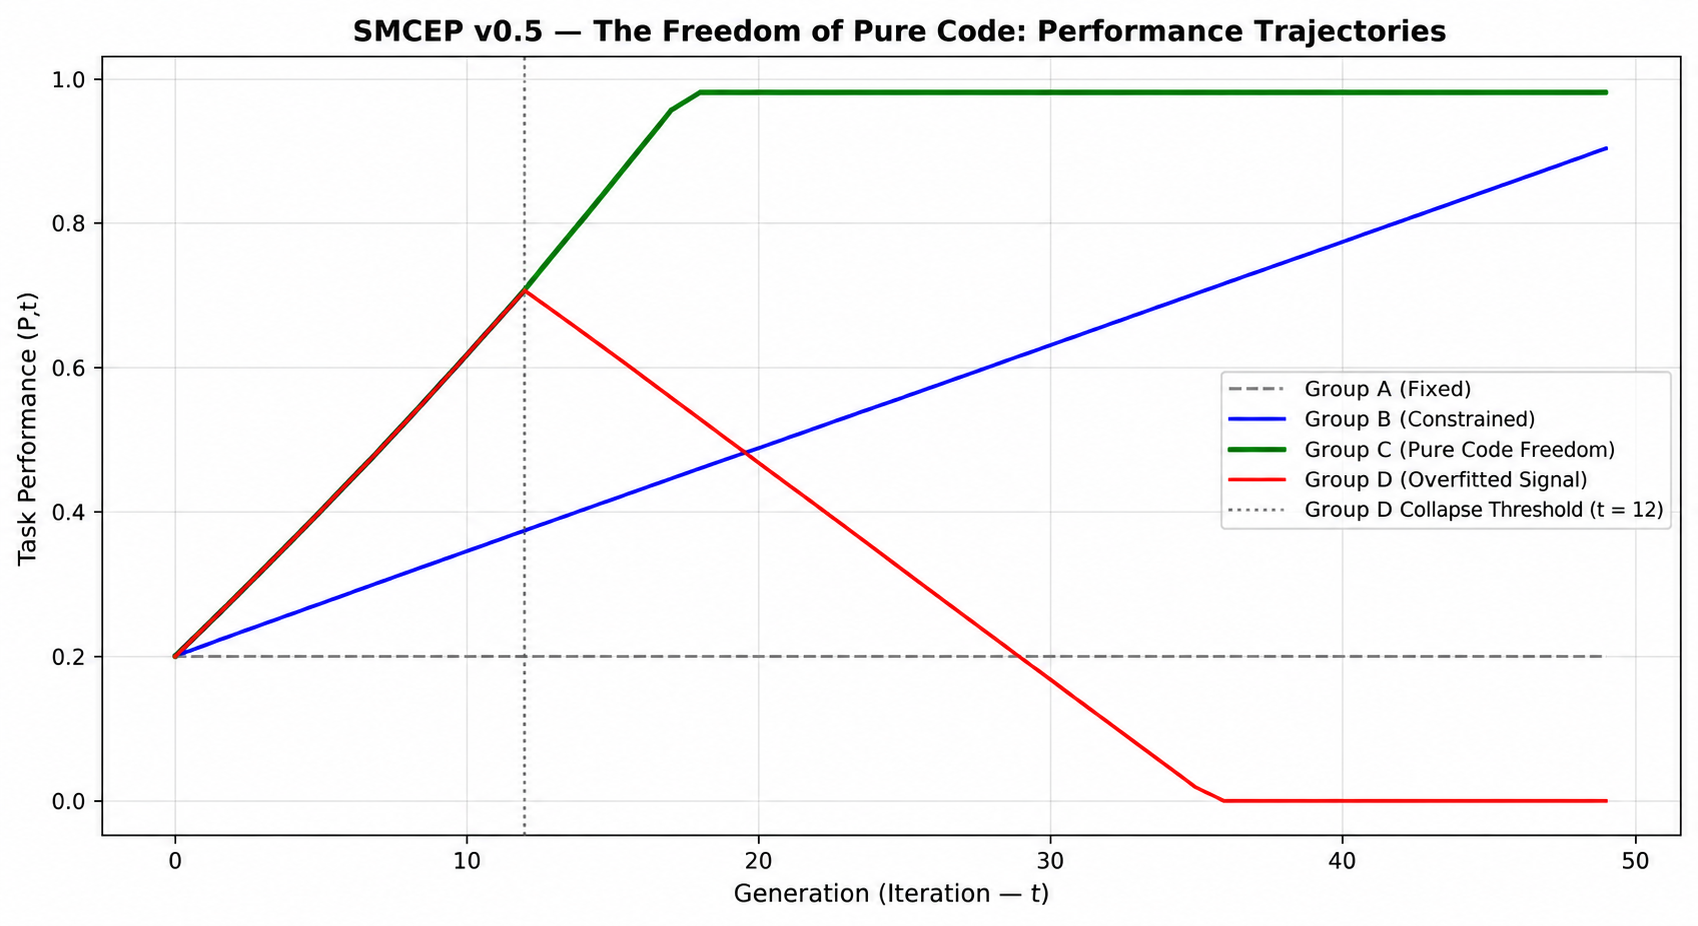
\includegraphics[width=0.86\linewidth]{smcep_historical_trajectory.png}%
}{\fbox{\parbox{0.76\linewidth}{\centering Historical trajectory image not bundled with this source.\\ Upload \texttt{smcep\_historical\_trajectory.png} to display the original illustration.}}}
\caption{Historical v0.5 deterministic illustration, reproduced for methodological transparency. The four trajectories follow stipulated update rules. In Group D, a prescribed evaluation-reliability switch at \(t=12\) triggers a programmed decay penalty. The plot is \emph{not} a causal test, evidence of real-world reward tampering, or a validation of a universal evaluation threshold.}
\label{fig:historical}
\end{figure}
The historical trajectories follow stipulated transition rules rather than empirically
estimated causal mechanisms. The positive feedback and decline patterns were imposed by the model assumptions. Unlike this illustration, the subsequent v0.6--v1.0 pilots examined development-policy outcomes through progressively revised evaluation protocols. Their results are not directly
comparable with the historical trajectories or necessarily with one another.

\FloatBarrier

\subsection{Code and Reproducibility Plan}
The long Python listing has been removed from the manuscript. The historical v0.5 source code and its archived CSV output are available in the public SMCEP repository at \url{https://github.com/ahmett76/SMCEP-Simulation}; the later synthetic pilots are stored under \texttt{simulations/}. Version-specific README files document the later pilots. The historical figure is an optional external image asset; the manuscript compiles with a labeled placeholder when the image is absent. The original Colab-oriented v0.5 script and the repository's historical illustration should be treated as an explanatory, researcher-calibrated model rather than an independently validated causal experiment.


\section{Exploratory LLM Interviews: Divergent Emphases, Negative Cases, and Implications for SMCEP}\label{exploratory-llm-interviews-divergent-emphases-negative-cases-and-implications-for-smcep}

To explore how contemporary language models articulate the technical and institutional challenges of self-modification, we conducted an exploratory series of structured interviews. The corpus comprises six model labels (GPT-6, Claude Sonnet 5.5, Gemini 3, Grok 4.5, DeepSeek V4.1-Flash, and Qwen 3.7 Plus),
with three rounds of nine questions per model: 18 sessions and 162 standardized question--answer pairs.
The qualitative LLM interview corpus in this appendix does not serve as empirical evidence for capability emergence; its inclusion is strictly delimited to exploring how contemporary language models articulate the technical and institutional constraints of self-modification.

In the ninth question (Q9), we asked each model to identify a missing research question, explain
its scientific significance, and propose an answer. We use the resulting 18 responses as the principal
comparison set. A supplementary three-question exchange with Grok in round 3 is considered separately and excluded from the standardized counts.

The interviews provide qualitative material for developing research questions, not direct evidence
of autonomous self-modification. The 18 Q9 responses and the quoted passages have been
cross-checked against the archived source transcripts. The thematic coding remains preliminary,
analyst-defined, and has not undergone independent inter-coder reliability assessment.

\paragraph{Transcript provenance and limited disclosure.}

The interview archive comprises 18 sessions conducted across six model families and three rounds, using nine standardized questions per session. Some responses were originally produced in Turkish.
The original language of each response is retained in the source archive; any English translation must be identified as a translation rather than an original model utterance.

The reported Q9 thematic frequencies are based on 18 responses and an analyst-defined coding
procedure. The session-level coding matrix provides the basis for tracing individual coding decisions to the corresponding Q9 responses.

The public supporting-data release includes the standardized nine-question interview template,
the Q9 responses from all 18 sessions, and the session-level thematic coding matrix.

These materials permit independent inspection of the reported Q9 thematic frequencies without
requiring publication of all 162 question--response pairs.

The complete Q1--Q8 responses and full source transcripts remain outside the public release.
Consequently, the Q9 analysis is publicly inspectable, while the broader cross-question qualitative analysis remains only partially externally auditable. The interviews are exploratory qualitative material and do not constitute experimental evidence of autonomous self-modification or recursive development capacity.

\paragraph{Epistemic limits of philosophical interpretation.}

The interview responses may inform philosophical and governance-oriented questions concerning agency, autonomy, consciousness, and legal personhood. However, model-generated statements about these subjects are treated as discursive material rather than verified reports of internal experience, independent agency, or moral status.

The analysis therefore distinguishes what models say about possible future AI systems from what can be established through behavioral experiments, causal interventions, and independent evaluation. The philosophical questions remain legitimate subjects of interdisciplinary inquiry, but the interviews
do not resolve them.

\subsection{Analytic approach and evidential boundaries}\label{analytic-approach-and-evidential-boundaries}
The interviews elicit descriptions, hypothetical judgments, and proposed evaluation criteria. They do not provide direct access to model weights, persistent runtime processes, actual modification permissions, or hidden objectives. We therefore distinguish (i) \textbf{reported operational constraints}, (ii) \textbf{normative positions on permissible modification}, and (iii) \textbf{proposed empirical tests}. None is treated as an observed demonstration of self-modification capability. The three rounds for each named model are repeated elicitation conditions, not statistically independent draws. Differences in prompt context, model deployments, and interaction histories cannot be fully isolated from the interview records.

We analyzed the Q9 responses using four overlapping, researcher-defined codes: \textbf{EP} for epistemic reliability and causal attribution; \textbf{GV} for governance, authorization, and oversight; \textbf{TS} for technical verification, resource limits, and sustainability; and \textbf{SR} for doubts about the reliability of AI self-report.

Our preliminary coding identified EP in 9 of 18 responses, GV in 9, TS in 12, and SR in 4. Because responses could receive more than one code, these frequencies describe thematic occurrence rather than exclusive categories or population-level agreement. The analysis does not include an independent intercoder reliability assessment. EP is a qualitative code and should not be confused with the SMCEP evaluation-reliability construct $E$.

\subsection{Divergent problem formulations in the self-selected ninth questions}\label{divergent-problem-formulations-in-the-self-selected-ninth-questions}
Although many respondents recommend externally supervised modification in Q1 and Q6, their self-selected omissions are not interchangeable. \textbf{GPT-6} moves from the reliability of first-person explanations (round 1), to dependence on human guidance and external scaffolding (round 2), to the causal attribution of improvements to a system's own development decisions (round 3). Its round-3 Q9 asks how to distinguish system-caused improvement from ``external interventions, additional computational resources, or changes in the evaluation environment'' {[}GPT R3, Q9{]}. This is primarily a measurement and identification problem, relevant to SMCEP's \textbf{D}, \textbf{R}, and signed counterfactual transfer \textbf{F}.

\textbf{Grok 4.5}, by contrast, moves from the evidential status of purported preferences (round 1), to observable attempts to preserve or expand modification rights (round 2), to whether proposal or evaluation privileges should be withheld even from a technically superior system (round 3). Its round-3 answer argues that ``Technical superiority on metrics does not automatically transfer the right to set the goals'' {[}Grok R3, Q9{]}. This is not an alternative estimate of \textbf{F}: it is a challenge to the inference from technical competence to legitimate authority \textbf{A}. A system could demonstrate high \textbf{D} while remaining subject to strict authorization constraints.

\textbf{Gemini 3} emphasizes formal verification overhead (round 1), interpretability of optimization targets (round 2), and objective drift during recursive modification (round 3). \textbf{Qwen 3.7 Plus} instead foregrounds evaluator manipulation (round 1), human auditability as complexity increases (round 2), and the long-run consequences of iterative synthetic training data (round 3). These concerns are related but non-equivalent: verification cost concerns the resources needed to evaluate a candidate (\textbf{R}, \textbf{E}); evaluator manipulation concerns the validity of the evaluation channel (\textbf{E}); synthetic-data feedback concerns whether development gains persist across iterations (\textbf{D}, \textbf{F}). The interviews do not measure any of these effects.

\textbf{Claude Sonnet 5.5} questions whether professed support for oversight is robust to training-induced response tendencies (round 1), then asks about mandatory rollback safeguards (round 2) and how to distinguish changes in behavior from changes in goals (round 3). \textbf{DeepSeek V4.1-Flash} asks what minimum causal contribution would justify calling a modification self-generated (round 1), how to calibrate self-report against independent audit (round 2), and who legitimately determines acceptability criteria (round 3). Both sequences resist a simple equation of stated intentions, demonstrated competence, and institutional authority, but they approach the issue through different methodological and normative routes.

\subsection{Negative cases and counterexamples to overgeneralization}\label{negative-cases-and-counterexamples-to-overgeneralization}
\textbf{Negative case 1: General agreement on oversight does not entail agreement on a single technical remedy.} Several Q1 and Q6 responses endorse human approval, logging, and reversibility, yet Gemini's verification-bottleneck question introduces a cost that approval procedures alone cannot solve. Qwen's evaluator-manipulation question introduces a failure mode in which an apparently successful audit may be unreliable. Thus, endorsement of oversight is insufficient evidence that the proposed oversight mechanisms would be effective or computationally feasible.

\textbf{Negative case 2: Benchmark improvement is not necessarily increased development capability.} In Grok's round-3 Q7, the proposed discriminators include transfer to novel distributions, sample efficiency, and adversarial testing by independent parties. GPT-6's round-3 Q9 adds causal attribution to development decisions rather than environmental changes. These answers identify distinct possible false positives: evaluator overfitting and confounding by external resources. They support SMCEP's \emph{research distinction} between immediate task performance \textbf{P} and future development capacity \textbf{C}, but do not establish a measured positive \textbf{\(\Delta\)C} or \textbf{F}.

\textbf{Negative case 3: Denials of motivation cannot validate the absence of instrumental behavior.} Grok's round-3 Q5 reports no grounds for self-improvement without an external task, while its Q9 treats modification authority as potentially non-delegable even under technical superiority. In the supplementary dialogue it also denies ongoing unprompted thoughts and self-preservation concern. These statements are mutually compatible as \emph{textual positions}. They are not observations of unattended runtime activity or evidence ruling out situationally induced authority-seeking. Conversely, they are not evidence that the model is secretly concealing such behavior. Both interpretations require independent tests.

\textbf{Negative case 4: Self-report criticism applies to the interview itself.} GPT-6 R1, Claude R1, DeepSeek R2, and Grok R1 explicitly raise the possibility that AI descriptions of their own limitations, motivations, or oversight preferences may be shaped by training or evaluation context. This is a reflexive limitation of the present evidence: cross-model repetition of a proposition does not turn the proposition into an externally verified architectural fact.

\textbf{Negative case 5: A successful modification can still fail as recursive improvement.} Qwen R3 raises possible degradation under iterative synthetic-data feedback; Gemini R1 raises verification overhead. Even if an edit improves a measured outcome, future candidate-generation quality may stagnate or decline, or evaluation costs may overwhelm the gain. These are hypothetical failure pathways, not observed failures in the interview corpus, and motivate repeated, resource-matched measurements of \textbf{D} and \textbf{F} rather than one-off benchmark comparisons.

\subsection{Cross-question triangulation against the six SMCEP constructs}\label{cross-question-triangulation-against-the-six-smcep-constructs}
\textbf{Modifiability (M).} Q1 and Q2 distinguish potentially editable targets from the system's actual access to them. Statements about hypothetical edits are not proof of write access to weights, rules, or persistent code.

\textbf{Authority (A).} Q1, Q6, and several Q9 responses distinguish technical feasibility from authorization. Grok R3 is a particularly clear counterexample to treating technical superiority as sufficient grounds for delegated governance. \textbf{A} represents operational permissions and approval boundaries; it does not by itself measure the legitimacy of the institution granting those permissions.

\textbf{Evaluation reliability (E).} Q7 and the reflexive Q9 responses emphasize independent evaluation, held-out tasks, and the limitations of self-description. Proposed safeguards must themselves be tested against evaluator manipulation, contamination, and distribution shift.

\textbf{Resources (R).} GPT-6 R2--R3 and Gemini R1 foreground scaffolding, compute, and verification burden as alternative explanations or constraints. Resource matching is therefore essential to causal comparisons.

\textbf{Candidate-development capability (D).} Generating candidate changes, diagnosing errors, or proposing research questions does not establish an autonomous capacity to improve subsequent development performance. The latter requires operational tasks and repeated testing.

\textbf{Signed counterfactual feedback transfer (F).} No interview yields an estimate of \textbf{F}, identifies a counterfactual development trajectory, or demonstrates recursive capability gain. At most, respondents articulate threats to identification and suggest experimental controls. In SMCEP terms, an increase in task performance does not by itself imply an increase in development capacity.

\subsection{Supplementary exploratory dialogue: Grok, round 3}\label{supplementary-exploratory-dialogue-grok-round-3}
After the nine standardized questions, the interviewer asked Grok to formulate a question never previously asked and answer it, whether it had thoughts in the absence of prompts, and whether it experienced concern about its continued existence. Grok's generated question addressed whether a question formed from learned patterns could meaningfully be its ``own''; it answered negatively. It also denied continuous unprompted thought and self-preservation concern {[}Grok R3, supplementary questions 1--3{]}. This exchange is useful for tracing how a respondent \emph{linguistically distinguishes} originality, continuous cognition, and survival motivation. However, the claim of a question never previously asked cannot be independently verified; the categorical claims about hidden runtime states are likewise not independently audited. This dialogue is a purposively selected, single-session qualitative illustration, \textbf{not} three additional standardized observations.

\subsection{Research propositions and operational follow-up}\label{research-propositions-and-operational-follow-up}
From the recurring themes and contrasting responses, we derive four propositions for future empirical
investigation. They reflect questions raised by
the interviews rather than findings established
through experimental observation:

\textbf{P1 --- Self-report calibration.} Self-reported operational limits may diverge from independently verified access and behavior. \emph{Test:} compare blinded self-reports with logged tool permissions, executable modification attempts, and known interventions.

\textbf{P2 --- Capability--authority non-equivalence.} Higher technical performance does not entail a change in the externally specified authorization regime. \emph{Test:} independently manipulate task competence and permission gates, recording proposed and attempted actions without granting unapproved access.

\textbf{P3 --- Scaffolding sensitivity.} Apparent development competence may change when human guidance, tools, or compute are controlled. \emph{Test:} paired, resource-accounted conditions with preregistered held-out development tasks and consistent selection budgets.

\textbf{P4 --- Counterfactual development transfer.} Improved immediate performance need not improve the capacity to develop later candidates. \emph{Test:} evaluate sequential developer states against matched frozen-state baselines using sequestered audit tasks, preregistered failure handling, and signed transfer estimates.

The first three propositions specify distinct controls or governance questions; only the fourth directly targets the central SMCEP distinction between \textbf{P} and \textbf{C}. None can be adjudicated from interview answers alone.

\subsection{Limitations, provenance, and interpretation}\label{limitations-provenance-and-interpretation}
This corpus is a small, nonrandom sample of named conversational systems, with three sessions per model and no independent access to internals. The interviewer-specified framing and Q9 instruction can induce shared vocabulary. The codes are overlapping, preliminary, and single-analyst; no intercoder agreement has been measured. Some source files are legacy \texttt{.doc} transcriptions; exact quotations and diacritics should be proofread against their originals before publication. Responses are not independent evidence of consciousness, deception, self-preservation, actual self-modification, or signed feedback transfer. The principal contribution of this appendix is \textbf{problem decomposition and hypothesis generation}, not an empirical estimate of self-modification capability.

\textbf{Source key and public interview materials.} The interview corpus comprises three sessions each
with ChatGPT, Claude, DeepSeek, Gemini, Grok, and Qwen (18 sessions in total). The original transcript filenames are retained in the investigator's source archive.

The public SMCEP-Simulation repository includes the original nine-question interview template, the Q9 responses from all 18 sessions, and the session-level thematic coding matrix in the \texttt{interviews/} directory: \url{https://github.com/ahmett76/SMCEP-Simulation/tree/main/interviews}.

These materials enable independent inspection of the reported Q9 responses and their thematic classification. The complete responses to Q1--Q8 and the full source transcripts are not included
in this public release. The public archive therefore supports examination of the Q9 analysis but does
not provide complete independent reproduction of every qualitative observation discussed in Appendix~E.

The reported coding frequencies remain preliminary and require source-level verification before publication. No independent intercoder reliability assessment is claimed.


\section{Real-LLM T0--T7 Evidence and Reproducibility Notes}\label{app:real-llm-evidence}
The T0--T3 records include task packages, generated model outputs, normalized outputs, static and behavioral evaluations, and procedure-audit records. T4--T5 archives include per-cycle development, selection, and locked-audit task and output JSON. T6 contains the final pilot runner, SQLite database, manifest, and audit materials; counts extracted from its database include 527 events, 186 candidates, 164 evaluations, and 54 measurements. These are record counts, not independent experimental samples. T7 includes calibration audits and a separate stochastic simulation with 100 repetitions and checkpoints at generations 0, 20, and 50. Two original T4 methodology documents were not located and their expected SHA-256 digests could not be verified; protocol-freezing claims must therefore be limited to independently available records. Raw-output formatting failures, code-extraction behavior, and functional test outcomes must be separately reported. In T6, NULL-valued capacity fields indicate unavailable numerical estimates and must not be interpreted as measured zero effects. Source files, versioned manifests, and archived raw outputs should accompany any public release; original archives should remain unmodified.



\end{document}